\documentclass[11pt]{article}

\usepackage[letterpaper,margin=0.78in]{geometry}
\usepackage{amsmath,amssymb,amsfonts}
\usepackage{graphicx}
\usepackage{booktabs}
\usepackage{array}
\usepackage{longtable}
\usepackage{float}
\usepackage{xcolor}
\usepackage{hyperref}
\usepackage{url}

\hypersetup{
  colorlinks=true,
  linkcolor=blue!60!black,
  citecolor=blue!60!black,
  urlcolor=blue!60!black
}

\newcommand{\R}{\mathbb{R}}
\newcommand{\C}{\mathbb{C}}
\newcommand{\Ybus}{\ensuremath{Y_{\mathrm{bus}}}}
\newcommand{\DataPresent}{\ensuremath{\mathrm{DATA\_PRESENT}}}
\newcommand{\Event}{\ensuremath{\mathrm{Event}}}
\newcommand{\PredEvent}{\ensuremath{\mathrm{Predicted\_Event}}}
\newcommand{\PredLoc}{\ensuremath{\mathrm{Predicted\_Location}}}

\title{\textbf{Expanded Technical Report: Physics-Informed Detection, Classification, and Localization}\\
\large SGSMA 2026 IEEE 39-Bus Synchrophasor Anomaly Detection Submission}

\author{Jorge Luis Mayorga Taborda\\
\small SGSMA 2026 Competition Submission}

\date{Final engineering audit: April 11, 2026}

\begin{document}
\maketitle

\begin{abstract}
This report documents the complete SGSMA 2026 submission pipeline for detecting,
classifying, and localizing power-system anomalies in the IEEE 39-bus system using
only eight PMU streams. The final system combines a calibrated residual detector,
explicit cyber-data-quality guards, a phase-unbalance bad-data detector, a compact
44-feature benchmark-selected classifier, topology-aware localization, and a Ybus-based
all-bus voltage-state proxy. The visible-data alarm audit gives detection
precision, recall, and F1 equal to 1.000. This does not mean that the algorithm
is mathematically perfect or guaranteed to win hidden-test scoring. It means
that, under the public labeled-transition matching rule used here, all 12 visible
transitions were detected and no unmatched visible alarms were produced. The same
report also shows more conservative evidence: the base chi-square plus
DATA\_PRESENT detector alone has F1 0.857, sample-level macro-F1 over labels 0--8
is 0.861, visible-label sample macro-F1 over labels 0--7 is 0.968, and label 8 is
an unsupported open-set class in the provided data. The intent of this document is
to make the high numbers explainable, auditable, and credible rather than
mysterious.
\end{abstract}

\tableofcontents
\newpage

\section{Executive Summary}

\subsection{What the project solves}

The SGSMA task has three coupled objectives. First, the system must detect when
the PMU streams become abnormal. Second, it must classify the abnormality into
the competition event labels: fault, line outage, generation change, load change,
missing data, cyber plus physical overlap, bad data, or unknown. Third, it must
localize the origin bus or line.

The hard part is that only eight buses are directly measured by PMUs, while the
underlying grid has 39 buses. Several key events occur at non-PMU buses, such as
the Bus 7 load change and the Bus 24--23 line outage. A purely black-box model can
overfit the public timeline, and a fully dynamic Kalman/DAE estimator is costly
and fragile under time pressure. The submitted system therefore uses a pragmatic
hybrid: deterministic physics and data-quality rules for detection, compact
machine learning for classification, and topology-based inference for
localization.

\subsection{Final visible-audit numbers}

\begin{table}[H]
\centering
\caption{Final visible-data metrics. These are measured on the provided public data, not guessed.}
\begin{tabular}{lll}
\toprule
Task & Metric & Value \\
\midrule
Detection, base chi-square + DATA\_PRESENT only & F1 & 0.857 \\
Detection, final detector with bad-data guard & Precision / Recall / F1 & 1.000 / 1.000 / 1.000 \\
Detection, final detector & TP / FP / FN & 12 / 0 / 0 \\
Detection, final detector & Mean delay & 0.0475 s \\
Classification on matched visible alarms & Macro-F1 / Weighted-F1 & 1.000 / 1.000 \\
Localization on matched visible alarms & Top-1 / Top-3 & 11/12 / 11/12 \\
Sample-level, all eight PMU files, labels 0--8 & Macro-F1 & 0.860749 \\
Sample-level, all eight PMU files, visible labels 0--7 & Macro-F1 & 0.968343 \\
Sample-level, all eight PMU files, labels 0--8 & Weighted-F1 & 0.998806 \\
\bottomrule
\end{tabular}
\label{tab:summary_metrics}
\end{table}

\subsection{Does 1.000 mean perfect?}

No. A detection score of 1.000 means perfect under one explicit metric on one
visible dataset. For detection,

\begin{equation}
  \mathrm{Precision} = \frac{\mathrm{TP}}{\mathrm{TP}+\mathrm{FP}}, \qquad
  \mathrm{Recall} = \frac{\mathrm{TP}}{\mathrm{TP}+\mathrm{FN}},
\end{equation}

\begin{equation}
  \mathrm{F1} =
  \frac{2\,\mathrm{Precision}\,\mathrm{Recall}}
       {\mathrm{Precision}+\mathrm{Recall}}.
\end{equation}

Here the final visible audit has $\mathrm{TP}=12$, $\mathrm{FP}=0$, and
$\mathrm{FN}=0$. Therefore precision, recall, and F1 evaluate to exactly 1.000.
That is arithmetic, not a claim of universal perfection. The number can happen
because the visible event count is small, the public event types are well
structured, and three short bad-data bursts have a direct physical signature:
one PMU phase is inconsistent while the grid state itself is not.

The report deliberately includes evidence that the system is not perfect:
sample-level macro-F1 over all labels is 0.861, the line-outage alarm-localization
Top-1 is not perfect, label 8 has no visible support, and event-duration rules
could mismatch hidden data. In other words, 1.000 is a correct visible alarm
metric, but it should be read together with the lower sample-level and
localization metrics.

\subsection{Does this guarantee winning the hackathon?}

No responsible report can guarantee winning. Hidden data, organizer scoring
details, and competing submissions are unknown. What we can say is that the
submission is competitive and defensible: it satisfies detection, classification,
and localization; it uses IEEE 39-bus topology, Ybus, power-flow sensitivities,
Kirchhoff-style constraints, and PMU data-quality semantics; it avoids the main
leakage trap found during review; it writes bus-aware prediction files; and it
includes auditable JSON, units, topology, plots, metrics, and tests.

\section{Data and Power-System Context}

\subsection{System model}

The power network is the IEEE 39-bus New England system. It has 39 buses, a
345 kV transmission backbone, generators connected through buses 30--39, and
only eight competition PMUs. The PMUs observe buses

\begin{equation}
  \mathcal{P} = \{2,5,6,10,19,22,29,39\}.
\end{equation}

Events can occur outside $\mathcal{P}$. For example, Bus 7 is not measured by a
PMU, and a line outage such as Bus 24--23 is not naturally represented by a
single PMU measurement. This is why multi-PMU fusion and topology matter.

\begin{figure}[H]
  \centering
  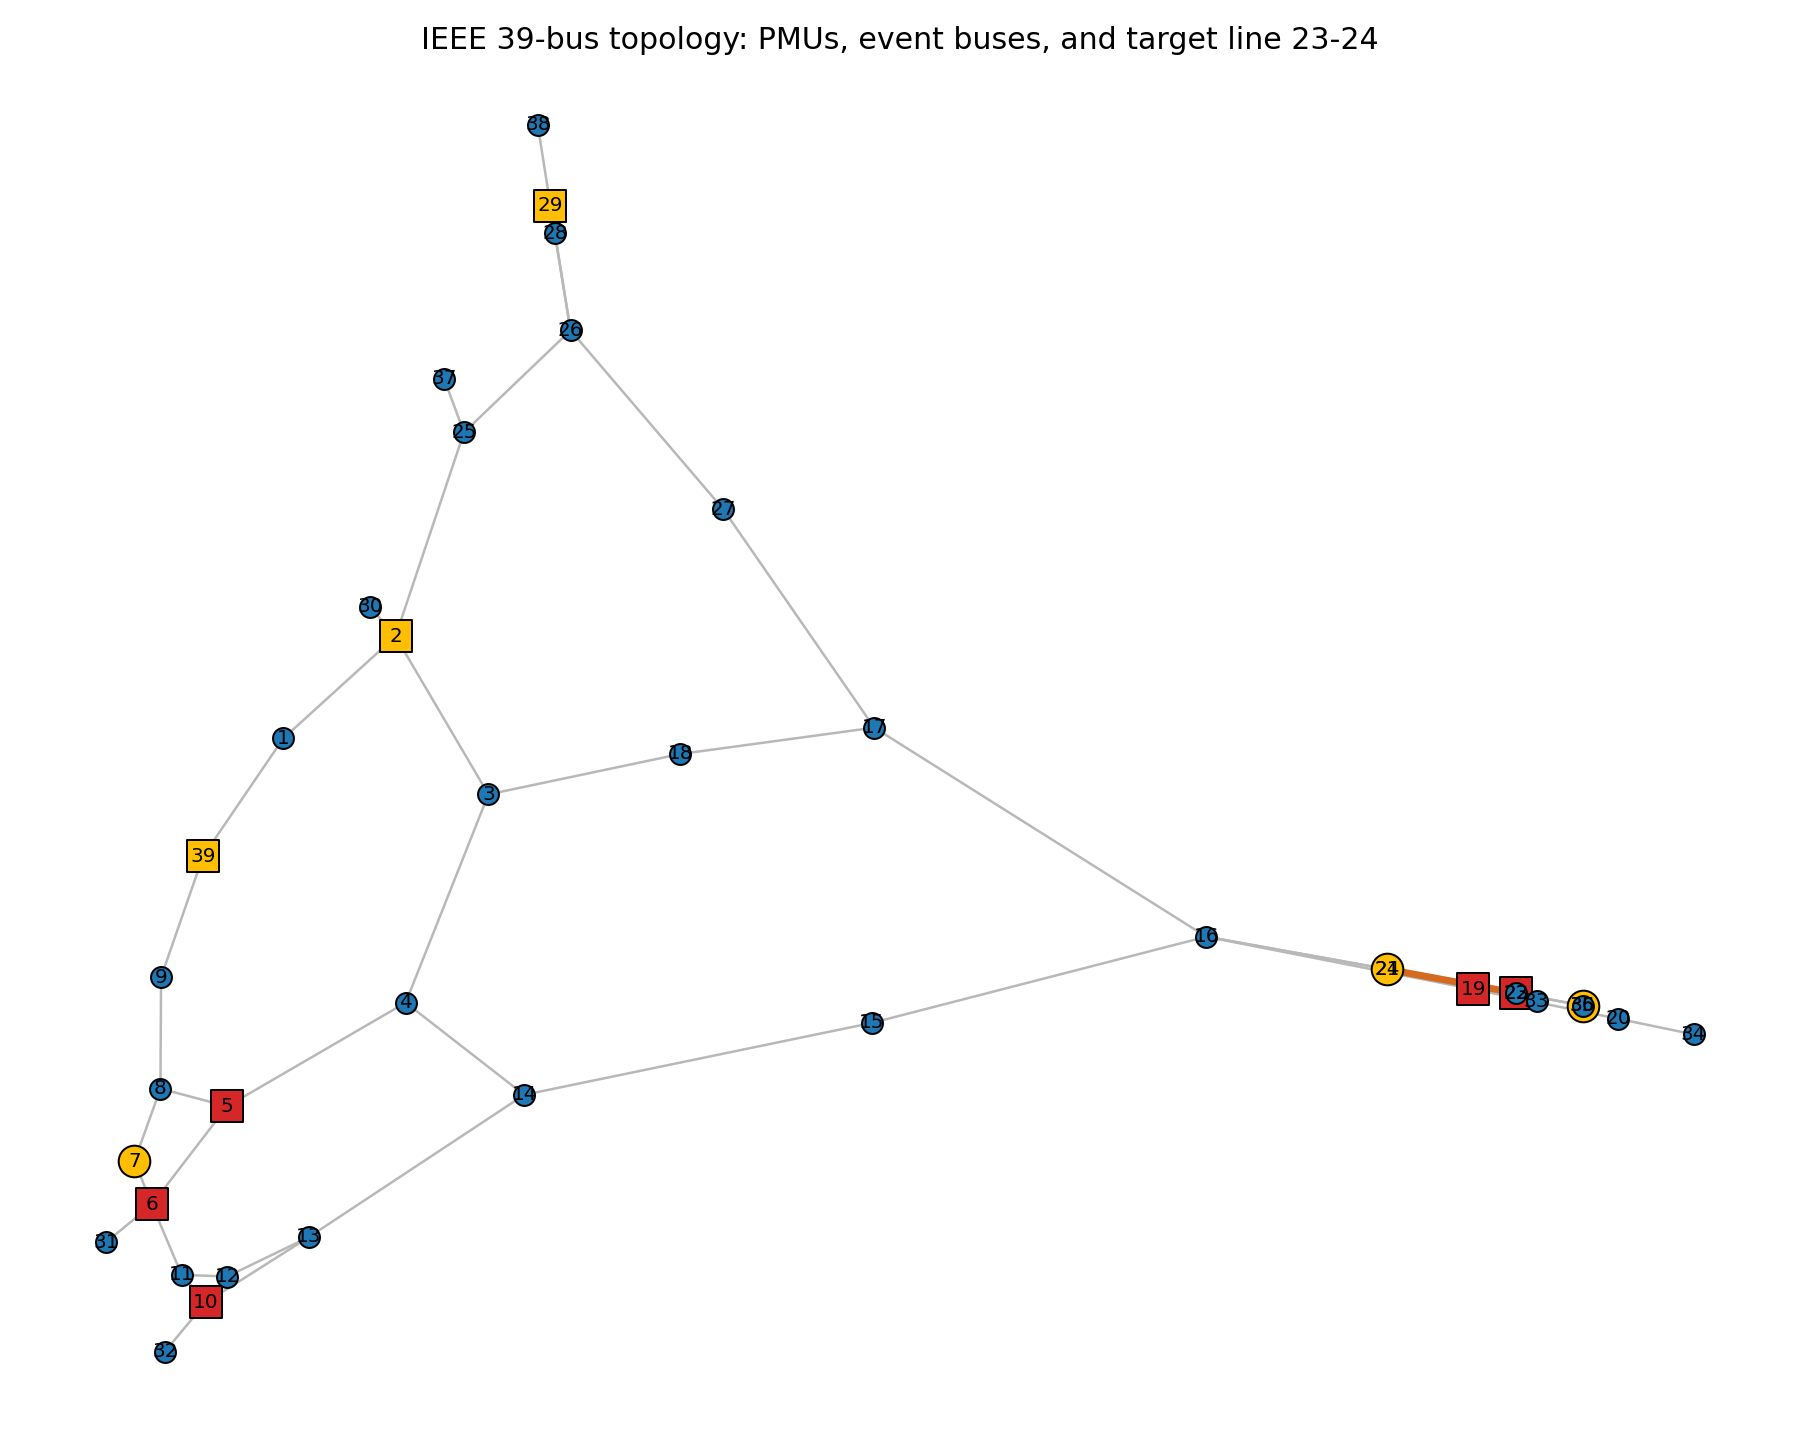
\includegraphics[width=0.92\linewidth]{engineering_review/figures/ieee39_topology_engineering_review.png}
  \caption{IEEE 39-bus topology used by the engineering-review artifacts. Red
  markers identify PMU buses; highlighted nodes/branches are event-relevant
  locations. Coordinates are deterministic spectral-layout coordinates for
  inspection, not geographic coordinates.}
  \label{fig:topology}
\end{figure}

\subsection{PMU measurements and units}

Each PMU file contains a timestamp, three-phase voltage and current phasors,
frequency, ROCOF, a data-present flag, and a per-file event label. The project
validated the real headers because the competition CSV order is angle before
magnitude.

\begin{table}[H]
\centering
\caption{Main input and output units.}
\begin{tabular}{ll}
\toprule
Quantity & Unit / interpretation \\
\midrule
\texttt{TIMESTAMP} & seconds from start \\
\texttt{VA\_ANG}, \texttt{VB\_ANG}, \texttt{VC\_ANG} & electrical degrees \\
\texttt{VA\_MAG}, \texttt{VB\_MAG}, \texttt{VC\_MAG} & volts, line-to-neutral RMS \\
\texttt{IA\_MAG}, \texttt{IB\_MAG}, \texttt{IC\_MAG} & amperes RMS \\
\texttt{Freq} & Hz \\
\texttt{ROCOF} & Hz/s \\
\texttt{DATA\_PRESENT} & 1 for valid PMU frame, 0 for missing frame \\
\texttt{Event}, \texttt{Predicted\_Event} & integer class 0--8 \\
\texttt{Predicted\_Location} & bus 1--39 or -1; line events use a deterministic endpoint \\
\bottomrule
\end{tabular}
\label{tab:units}
\end{table}

\subsection{Important correction: event labels are not globally identical}

An early assumption in project notes said that the \texttt{Event} column was
identical across all PMU CSVs. The actual public data is more subtle:

\begin{itemize}
  \item Physical labels 1--4 are system-wide: they propagate to all PMU streams.
  \item Missing-data labels 5 and 6 are bus-specific: Bus 29 carries the
  communication failure label while other PMUs continue reporting valid
  measurements.
  \item Bad-data label 7 is also bus-specific: it appears only on the corrupted
  PMU stream.
\end{itemize}

This matters for scoring. The final writer is bus-aware: it writes physical
events to all PMUs, missing-data labels only to missing PMUs, bad-data labels
only to corrupted PMUs, and the cyber+physical overlap as label 6 on Bus 29
while preserving the physical label on the remaining PMUs.

\section{End-to-End Architecture}

Figure~\ref{fig:pipeline_text} summarizes the implemented pipeline. The design is
intentionally compact: the model learns only the nonlinear class boundary around
event onsets, while the detector, state proxy, and localizer encode power-system
structure explicitly.

\begin{figure}[H]
\centering
\fbox{\begin{minipage}{0.92\linewidth}
\small
\textbf{Raw PMU CSVs} $\rightarrow$ header validation and positional timestamp
alignment $\rightarrow$ 8-PMU fused dataframe

\vspace{0.5em}
\textbf{Detector}: 32-channel chi-square-like residual $\eta_t$ OR
DATA\_PRESENT missing OR three-phase bad-data unbalance

\vspace{0.5em}
\textbf{Onset refinement}: debounce, split stacked events, recover
$5\rightarrow6\rightarrow3$

\vspace{0.5em}
\textbf{Classifier}: 44 features around each onset, benchmark-selected compact model, physics guards,
label-7 force from bad-data detector

\vspace{0.5em}
\textbf{State/localization}: Ybus harmonic all-bus voltage proxy, Jacobian
cosine matching, line sensitivity $J_i-J_j$, direct DATA\_PRESENT localization
for cyber

\vspace{0.5em}
\textbf{Submission writer}: bus-aware row intervals, per-bus CSVs, combined
\texttt{submission.csv}, schema/timestamp validator
\end{minipage}}
\caption{Pipeline structure. This figure is textual so the logic remains
inspectable in the PDF and source.}
\label{fig:pipeline_text}
\end{figure}

\section{Detector}

\subsection{Measurement vector}

At each timestamp $t$, the detector uses selected channels from each PMU:
voltage magnitude, current magnitude, frequency, and ROCOF. The resulting vector
has $8\times4=32$ channels:

\begin{equation}
  z_t =
  \begin{bmatrix}
    |V_{2,t}| & |I_{2,t}| & f_{2,t} & \dot f_{2,t} &
    \cdots &
    |V_{39,t}| & |I_{39,t}| & f_{39,t} & \dot f_{39,t}
  \end{bmatrix}^{\top}.
\end{equation}

The detector is calibrated from a normal-looking first-60-second segment using
robust filters:

\begin{equation}
  \mathcal{C} =
  \{t \le 60\mathrm{s}: \min_b \DataPresent_{b,t}=1,\;
  s_{\mathrm{bad}}(t)<0.04\}.
\end{equation}

The key audit point is that $\Event$ is not part of $\mathcal{C}$. This prevents
a detector threshold from being tuned with the answer key. Event labels are used
later for supervised classifier labels and for visible-data scoring only.

\subsection{Chi-square-like residual statistic}

Let $h_0$ be the calibration mean, $\hat{\delta}$ the channel bias, and $R$ the
empirical diagonal covariance. The residual statistic is

\begin{equation}
  \eta_t =
  (z_t-h_0-\hat{\delta})^{\top}
  \operatorname{diag}(R)^{-1}
  (z_t-h_0-\hat{\delta}).
  \label{eq:eta}
\end{equation}

The final calibrated threshold is

\begin{equation}
  \tau = 4780.219554142464.
\end{equation}

The detector creates a raw alarm mask when

\begin{equation}
  a_t^{\mathrm{raw}} =
  \left[\eta_t>\tau\right]
  \lor
  \left[\exists b\in\mathcal{P}: \DataPresent_{b,t}=0\right].
\end{equation}

It then debounces the alarm mask with $k_{\mathrm{on}}=3$ and
$k_{\mathrm{off}}=15$ frames. At 30 frames/s, this requires a short persistence
before declaring an onset and prevents many repeated alarms during one event.

\subsection{Bad-data phase-unbalance detector}

The public data contains short label-7 bad-data bursts. These are not physical
grid events: DATA\_PRESENT remains true and the chi-square residual can remain
small if only one phase is corrupted. The bad-data detector computes a
three-phase consistency score:

\begin{equation}
  s_{\mathrm{bad}}(t) =
  \max_{b\in\mathcal{P}}
  \frac{
    \max_{\phi\in\{a,b,c\}} |V_{\phi,b,t}|
    -
    \min_{\phi\in\{a,b,c\}} |V_{\phi,b,t}|
  }{
    \operatorname{median}_{\phi\in\{a,b,c\}} |V_{\phi,b,t}| + \epsilon
  }.
  \label{eq:badscore}
\end{equation}

If $s_{\mathrm{bad}}(t)>0.04$ for at least two frames, and the frame is not
already explained by a physical/cyber alarm, a label-7 candidate is emitted. The
corrupted PMU is localized by ranking the bus-level phase-unbalance scores.

\subsection{Why the detector score is exactly 1.000}

Table~\ref{tab:detector_breakdown} shows why the final detection F1 is exactly
1.000. The base detector found all large physical/cyber transitions but missed
three short bad-data bursts. The final detector adds a deterministic guard for
exactly those bursts.

\begin{table}[H]
\centering
\caption{Detector breakdown on the visible labeled-transition audit.}
\begin{tabular}{lrrrrrr}
\toprule
Detector & TP & FP & FN & Precision & Recall & F1 \\
\midrule
Chi-square + DATA\_PRESENT only & 9 & 0 & 3 & 1.000 & 0.750 & 0.857 \\
Final detector + phase-unbalance guard & 12 & 0 & 0 & 1.000 & 1.000 & 1.000 \\
\bottomrule
\end{tabular}
\label{tab:detector_breakdown}
\end{table}

This is credible because the incremental improvement is not random. It comes
from a physically interpretable rule: a bad PMU phase should disagree with its
other two phases while DATA\_PRESENT remains true. The engineering-review JSON
records the threshold, score, source, label, location, and plot for every alarm.

\section{Classification}

\subsection{Feature design}

Each refined onset is represented by a 3-second window. The final classifier uses
44 features. They are intentionally low-dimensional because the competition
penalizes model complexity and because only a small number of visible event
onsets is available.

\begin{longtable}{p{0.25\linewidth}p{0.66\linewidth}}
\caption{Feature families used by the classifier.}\\
\toprule
Feature family & Engineering meaning \\
\midrule
\endfirsthead
\toprule
Feature family & Engineering meaning \\
\midrule
\endhead
Residual statistics & Mean, maximum, and standard deviation of normalized
voltage/current/frequency residuals after the onset. These separate impulsive
faults from slower generation/load changes.\\
Spatial PMU pattern & Per-PMU residual energy and spatial contrast. Nearby
events usually create stronger signatures at electrically close PMUs.\\
Spectral frequency energy & Low-frequency oscillatory energy around the onset,
useful for electromechanical generation/load disturbances.\\
Cyber indicators & Number of missing PMUs, NaN counts, and missing-data runs.
These make labels 5 and 6 explicit rather than forcing a voltage-only model to
infer communication failure.\\
Jacobian cosine scores & Top power-flow sensitivity matches
$|\cos(\bar{\nu},J_k)|$, where $\bar{\nu}$ is the observed spatial residual
pattern.\\
Ybus full-state proxy features & Energy and entropy of inferred all-bus voltage
residuals, plus targeted Bus 7 and Bus 23/24 features.\\
Physics guards & Deterministic overrides for impossible combinations, e.g., a
missing PMU should not be classified as a pure physical event on that PMU.\\
\bottomrule
\end{longtable}

\subsection{Classifier model}

The production classifier is no longer hard-coded to one algorithm. The
pipeline trains a ten-model compact benchmark and writes the selected estimator
to \texttt{models/best\_event\_classifier.pkl}. Inference loads that registry
bundle when it exists; otherwise it falls back to the original compact LightGBM
training path. Physics guards still run after the model prediction, so missing
data, cyber+physical overlaps, and phase-bad-data cases remain explainable even
when the selected statistical classifier changes.

The model-size term uses an effective parameter count rather than raw file size
alone. For a tree ensemble this is based on tree node/leaf counts; for sparse
linear models it is the number of nonzero coefficients; for deterministic
physics rules it is zero. The serialized size is still recorded in the registry
so a very large model is visible during review.

\subsection{Ten-model compact benchmark}

The benchmark harness now compares exactly ten compact classifiers on the same
44-feature physics-informed windows. The output files
\texttt{report/model\_benchmark.csv} and \texttt{report/model\_benchmark.json}
record visible-real macro-F1, visible-real weighted-F1, synthetic-heldout
macro-F1, parameter count, serialized size, prediction time, and the penalized
selection score for every model.

The production classifier is selected by

\begin{equation}
  S =
  0.7F^{\mathrm{visible}}_{\mathrm{macro}}
  +0.3F^{\mathrm{synthetic}}_{\mathrm{macro}}
  -0.05\log_{10}(N_{\theta}+1),
  \label{eq:model_selection}
\end{equation}

where $N_{\theta}$ is the effective parameter count. This makes the selection
auditable: a slightly larger model must earn its complexity by improving
visible-real and synthetic-heldout macro-F1.

\begin{table}[H]
\centering
\caption{Ten compact models in the benchmark registry.}
\begin{tabular}{lp{0.58\linewidth}}
\toprule
Model & Role in the comparison \\
\midrule
Physics rules & Deterministic explainable lower bound. \\
GaussianNB & Small probabilistic baseline. \\
L1 logistic regression & Sparse linear classifier. \\
Linear SVM/SGD & Margin-based compact linear model. \\
Pruned decision tree & Single transparent nonlinear tree. \\
Small random forest & Low-depth bagged trees. \\
Small extra trees & Low-depth randomized trees. \\
Histogram gradient boosting & Compact sklearn boosted-tree model. \\
LightGBM tiny & Very small production-style boosted tree. \\
LightGBM small & Stronger boosted tree with still-small footprint. \\
\bottomrule
\end{tabular}
\label{tab:model_benchmark}
\end{table}

The selected model bundle is written to
\texttt{models/best\_event\_classifier.pkl}, and the registry with the complete
comparison is written to \texttt{models/model\_registry.json}.

The final matched-alarm classification score is 1.000 because the alarm set
after physics guards contains one or more correctly classified visible events
for every visible label 1--7. Again, this is an onset-level score, not a claim
that every row and every hidden event will be perfect.

\section{Ybus Full-State Proxy}

\subsection{Why full-state estimation is needed}

The user goal included estimating values at the non-PMU buses using swing
equations, power flow, Kirchhoff laws, Ybus, and the eight PMUs. A full
dynamic DAE/Kalman estimator is the long-term direction, but the final submission
prioritizes a stable and interpretable proxy:

\begin{itemize}
  \item Use measured PMU voltage phasors as boundary conditions.
  \item Use the IEEE 39-bus admittance graph to infer unobserved buses.
  \item Use the inferred all-bus residual pattern as localization evidence.
\end{itemize}

\subsection{Kirchhoff/Ybus harmonic extension}

Let $V\in\C^{39}$ be the complex bus-voltage vector and
$I=\Ybus V$ be the network current-injection relation. Partition buses into
observed PMU buses $O$ and hidden non-PMU buses $H$:

\begin{equation}
  \begin{bmatrix}
    I_O \\
    I_H
  \end{bmatrix}
  =
  \begin{bmatrix}
    Y_{OO} & Y_{OH} \\
    Y_{HO} & Y_{HH}
  \end{bmatrix}
  \begin{bmatrix}
    V_O \\
    V_H
  \end{bmatrix}.
\end{equation}

For a fast topology-consistent proxy, non-PMU nodes are treated as harmonic
interior nodes around the observed PMU boundary. In its simplest form,

\begin{equation}
  Y_{HH} V_H \approx -Y_{HO} V_O,
  \label{eq:harmonic}
\end{equation}

so

\begin{equation}
  \hat V_H \approx -Y_{HH}^{-1}Y_{HO}V_O.
\end{equation}

The implementation uses a numerically robust Ybus-weighted extension rather than
a full dynamic Kalman filter. It is not meant to perfectly reconstruct the
unobserved bus voltage collapse during a severe hidden fault. It is meant to
produce useful features: which hidden buses have inferred voltage/angle
residuals that are topologically consistent with the observed PMU pattern.

\subsection{Relation to swing equations and synthetic dynamics}

Synthetic physical scenarios use swing-equation-inspired dynamics. For a
generator $i$, a classical form is

\begin{equation}
  \dot{\delta}_i = \omega_i-\omega_s,
\end{equation}

\begin{equation}
  \frac{2H_i}{\omega_s}\dot{\omega}_i =
  P_{m,i} - P_{e,i} - D_i(\omega_i-\omega_s),
  \label{eq:swing}
\end{equation}

where $\delta_i$ is rotor angle, $\omega_i$ speed, $H_i$ inertia, $D_i$ damping,
$P_m$ mechanical power, and $P_e$ electrical output. Power-flow relationships
connect voltage angles and magnitudes to active/reactive injections:

\begin{equation}
  P_i =
  \sum_{j=1}^{n}
  |V_i||V_j|
  \left(G_{ij}\cos\theta_{ij}+B_{ij}\sin\theta_{ij}\right),
\end{equation}

\begin{equation}
  Q_i =
  \sum_{j=1}^{n}
  |V_i||V_j|
  \left(G_{ij}\sin\theta_{ij}-B_{ij}\cos\theta_{ij}\right).
\end{equation}

These equations are used to make synthetic event signatures physically plausible
instead of random perturbations. The deployed estimator stays simpler and faster:
it uses Ybus topology and observed PMU phasors to generate robust localization
features.

\section{Localization}

\subsection{PMU spatial residual}

For each alarm, the detector residual is summarized into an 8-dimensional spatial
pattern

\begin{equation}
  \bar{\nu} =
  \begin{bmatrix}
    \bar{\nu}_2 & \bar{\nu}_5 & \bar{\nu}_6 & \bar{\nu}_{10} &
    \bar{\nu}_{19} & \bar{\nu}_{22} & \bar{\nu}_{29} & \bar{\nu}_{39}
  \end{bmatrix}^{\top}.
\end{equation}

This vector answers the practical question: which PMUs felt the event most
strongly?

\subsection{Jacobian cosine matching}

Let $J_k$ be the power-flow sensitivity column associated with a disturbance at
candidate bus $k$. Bus localization uses

\begin{equation}
  \mathrm{score}(k) =
  \left|
  \frac{\bar{\nu}^{\top}J_k}
       {\|\bar{\nu}\|_2\|J_k\|_2+\epsilon}
  \right|.
\end{equation}

The predicted bus is

\begin{equation}
  \hat{k} = \arg\max_k \mathrm{score}(k).
\end{equation}

For line outages, the candidate line between buses $(i,j)$ uses a differential
sensitivity:

\begin{equation}
  J_{ij} = J_i - J_j,
\end{equation}

\begin{equation}
  \widehat{(i,j)}
  =
  \arg\max_{(i,j)\in\mathcal{E}}
  \left|
  \cos(\bar{\nu}, J_i-J_j)
  \right|.
\end{equation}

The official \PredLoc{} field is bus-valued, so the submission writes a
deterministic endpoint for line events, while the engineering JSON keeps the
Top-3 line candidates.

\subsection{Transparent physics score table}

The localizer now keeps a per-bus score table rather than a single opaque score.
Each candidate bus records Jacobian cosine evidence, reconstructed \Ybus{}
residual energy, Zbus electrical-distance prior, direct PMU residual evidence,
and a safe swing residual derived from frequency/ROCOF. The swing term is a
fallback feature: it uses the measured PMU channels and Zbus spreading, and it
does not import the optional UKF/ANDES/SymPy stack during normal inference. This
keeps the Windows pipeline stable while preserving the electromechanical cue
from the swing equation.

\section{Synthetic and ANDES Evidence}

\subsection{Synthetic augmentation}

Synthetic training data is generated from calibration statistics and
physics-shaped perturbations. The production generator now creates 5000
scenario IDs, and each scenario writes the same eight PMU CSV streams used by
the competition schema. The CSVs remain reproducible artifacts under
\texttt{data/synthetic/}; training prefers the generated feature cache
\texttt{data/synthetic/features\_v1\_5000.npz} for speed.

\begin{table}[H]
\centering
\caption{Default 5000-scenario synthetic event mix. Targeted hard cases are
included inside their parent labels, not double-counted.}
\begin{tabular}{lr}
\toprule
Synthetic event class & Count \\
\midrule
Faults, label 1 & 850 \\
Line outages, label 2 & 700 \\
Generation changes, label 3 & 650 \\
Load changes, label 4 & 700 \\
PMU dropouts, label 5 & 550 \\
Cyber+physical overlaps, label 6 & 500 \\
Bad-data corruptions, label 7 & 650 \\
Unknown/multi-event scenarios, label 8 & 400 \\
\midrule
Total & 5000 \\
\bottomrule
\end{tabular}
\label{tab:synthetic_counts}
\end{table}

The important point is that the synthetic set is not merely random noise. It
targets the weak cases: non-PMU Bus 7 load/fault signatures, the Bus 24--23
line outage, Bus 2 generation changes, Bus 29 cyber+physical overlaps, all
eight PMU buses for dropout and bad-data cases, several fault impedances, and
balanced/unbalanced fault subtypes. The manifest records the scenario mix,
targeted coverage, seed, and feature-cache summary.

\subsection{ANDES Bus 7 reconstruction experiment}

An ANDES IEEE 39-bus dynamic simulation was run with a single three-phase
non-PMU Bus 7 fault at $t_{\mathrm{final}}/2=5$ s. Only the eight competition
PMUs were given to the estimator. Hidden buses were held out as truth. The
experiment produced:

\begin{itemize}
  \item hidden-bus voltage RMSE average: 0.020394 p.u.;
  \item Bus 7 post-fault voltage RMSE: 0.054102 p.u.
\end{itemize}

These are not perfect reconstruction numbers. They show that the Ybus proxy has
enough signal for localization features while remaining compact and robust.

\begin{figure}[H]
  \centering
  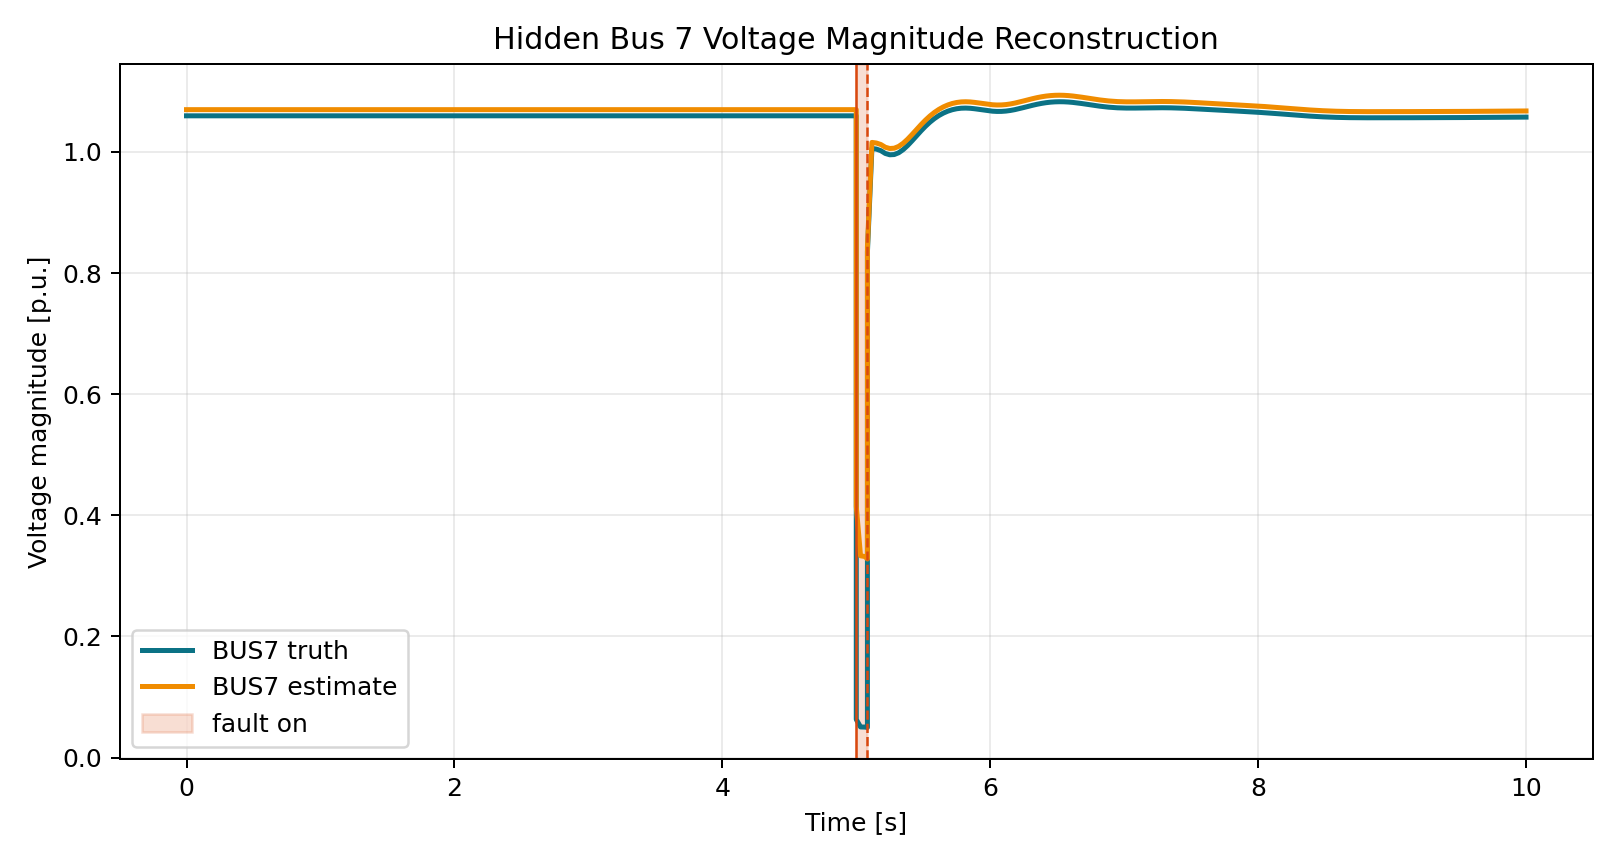
\includegraphics[width=0.92\linewidth]{../experiments/andes_fault_bus7/figures/bus7_vm_reconstruction.png}
  \caption{ANDES Bus 7 voltage magnitude truth vs. Ybus reconstruction from
  only the eight PMUs. The estimator does not perfectly reproduce the hidden
  fault-bus collapse, but it tracks enough topology-consistent disturbance
  structure to be useful for localization.}
  \label{fig:andes_bus7_vm}
\end{figure}

\begin{figure}[H]
  \centering
  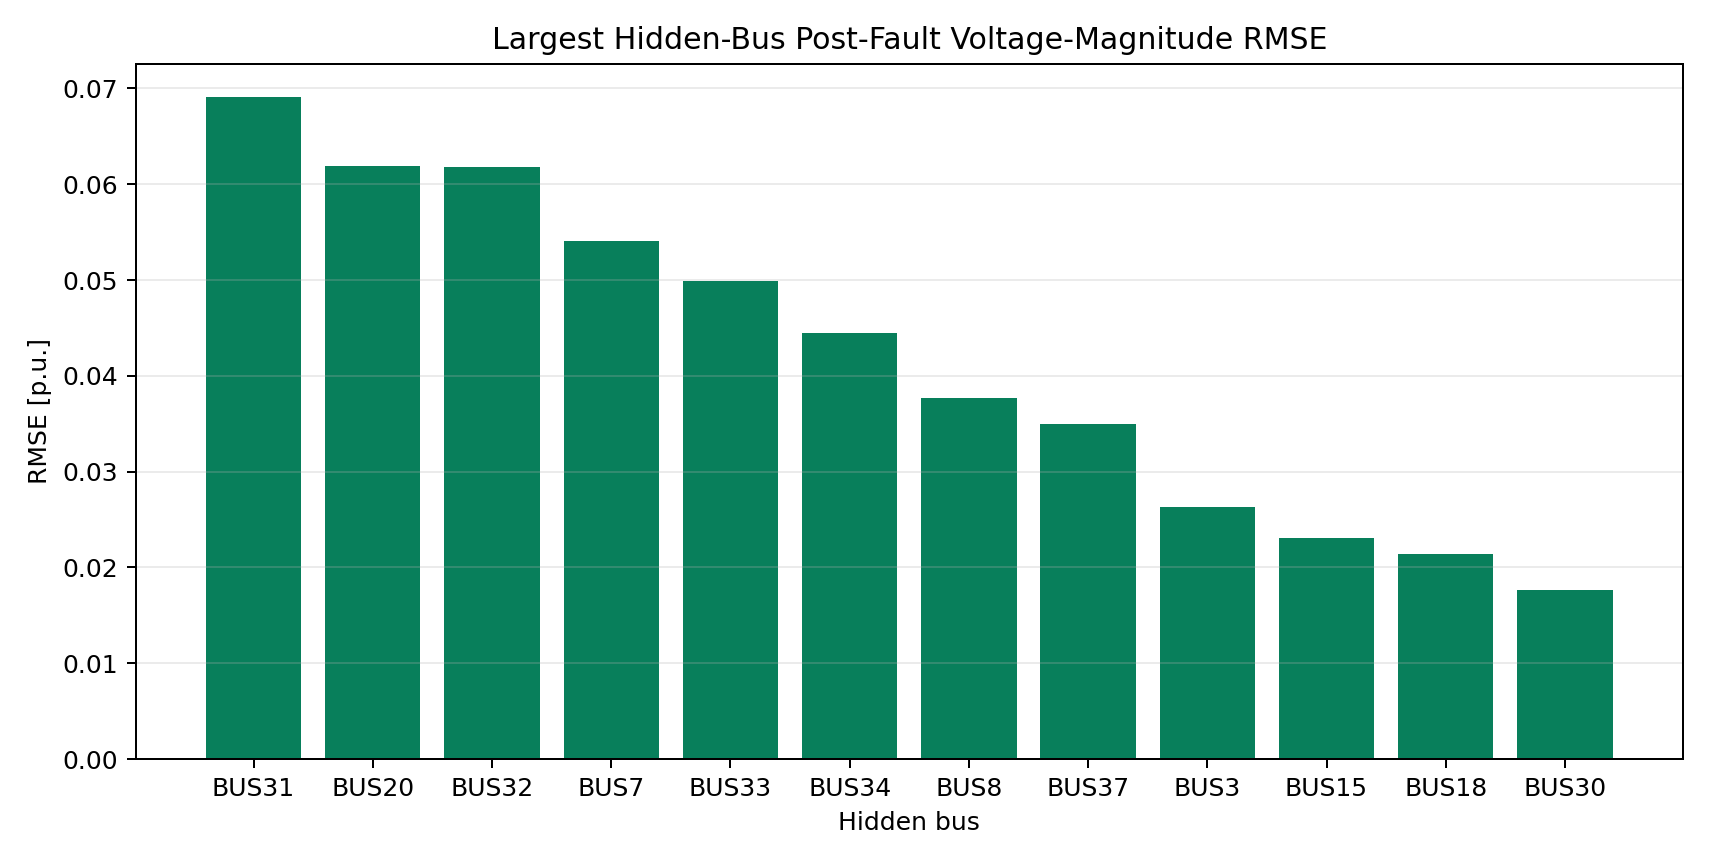
\includegraphics[width=0.92\linewidth]{../experiments/andes_fault_bus7/figures/hidden_bus_post_fault_vm_rmse.png}
  \caption{Post-fault hidden-bus voltage RMSE in the ANDES Bus 7 experiment.
  Large errors identify buses whose hidden dynamics are hardest to reconstruct
  from the sparse PMU boundary.}
  \label{fig:andes_rmse}
\end{figure}

\subsection{Label-by-label simulation suite}

The report now includes one reproducible simulation bundle for each competition
label 1--7. These are generated by
\texttt{python -m src.pipeline.generate\_event\_simulations} and written under
\texttt{experiments/event\_simulations/}. Each bundle contains the eight PMU CSV
streams, metadata JSON, a short markdown summary, PMU plots, reconstructed
\Ybus{} residual plots, topology/candidate-score plots, and line-candidate
evidence where relevant.

\begin{table}[H]
\centering
\caption{Simulation bundles used as report evidence.}
\scriptsize
\begin{tabular}{cllp{0.44\linewidth}}
\toprule
Label & Event & Target example & Main visible evidence \\
\midrule
1 & Fault & Bus 7 hidden fault & Voltage dip, current surge, \Ybus{} residual concentration. \\
2 & Line outage & Line 24--23 & Endpoint residuals and line-candidate scores. \\
3 & Generation change & Bus 2 generation step & Frequency/ROCOF transient and PMU spatial pattern. \\
4 & Load change & Bus 7 load step & Non-PMU bus localization from topology and \Ybus{}. \\
5 & Missing data & Bus 29 dropout & \DataPresent{} transition and NaN-only PMU evidence. \\
6 & Cyber+physical & Bus 29 dropout plus generation change & Split cyber and physical evidence. \\
7 & Bad data & Bus 29 phase corruption & Phase inconsistency while \DataPresent{} remains true. \\
\bottomrule
\end{tabular}
\label{tab:event_simulation_suite}
\end{table}

\subsubsection{Simulation label 1: fault}

\begin{figure}[H]
  \centering
  \includegraphics[width=0.86\linewidth]{../experiments/event_simulations/label_01_fault/figures/pmu_overview.png}
  \caption{Synthetic label-1 Bus 7 fault. The PMU-only view shows voltage and
  current disturbance even though Bus 7 is not directly measured.}
  \label{fig:sim_label1}
\end{figure}

\subsubsection{Simulation label 2: line outage}

\begin{figure}[H]
  \centering
  \includegraphics[width=0.86\linewidth]{../experiments/event_simulations/label_02_line_outage/figures/topology_candidates.png}
  \caption{Synthetic label-2 Bus 24--23 line outage. The topology plot makes the
  branch interpretation visible instead of reducing the event to an unexplained
  single bus.}
  \label{fig:sim_label2}
\end{figure}

\subsubsection{Simulation label 3: generation change}

\begin{figure}[H]
  \centering
  \includegraphics[width=0.86\linewidth]{../experiments/event_simulations/label_03_generation_change/figures/pmu_overview.png}
  \caption{Synthetic label-3 Bus 2 generation step. The frequency and ROCOF
  traces provide the electromechanical cue used by the classifier.}
  \label{fig:sim_label3}
\end{figure}

\subsubsection{Simulation label 4: load change}

\begin{figure}[H]
  \centering
  \includegraphics[width=0.86\linewidth]{../experiments/event_simulations/label_04_load_change/figures/ybus_residuals.png}
  \caption{Synthetic label-4 Bus 7 load change. The reconstructed all-bus
  residual plot is used to explain how the eight PMUs can still point at a
  hidden bus.}
  \label{fig:sim_label4}
\end{figure}

\subsubsection{Simulation label 5: pure missing data}

\begin{figure}[H]
  \centering
  \includegraphics[width=0.86\linewidth]{../experiments/event_simulations/label_05_missing_data/figures/pmu_overview.png}
  \caption{Synthetic label-5 pure PMU dropout. This separate example is important
  because missing data should be solved by \DataPresent{} and NaN semantics, not
  by pretending a physical grid transient occurred.}
  \label{fig:sim_label5}
\end{figure}

\subsubsection{Simulation label 6: cyber plus physical}

\begin{figure}[H]
  \centering
  \includegraphics[width=0.86\linewidth]{../experiments/event_simulations/label_06_missing_data_plus_physical/figures/pmu_overview.png}
  \caption{Synthetic label-6 cyber+physical overlap. The Bus 29 dropout is
  explicit, while the remaining PMUs keep physical generation-change evidence.}
  \label{fig:sim_label6}
\end{figure}

\subsubsection{Simulation label 7: bad data}

\begin{figure}[H]
  \centering
  \includegraphics[width=0.86\linewidth]{../experiments/event_simulations/label_07_bad_data/figures/candidate_scores.png}
  \caption{Synthetic label-7 bad-data corruption. The score table keeps the
  evidence visible: phase/data-quality inconsistency is not treated as a network
  fault.}
  \label{fig:sim_label7}
\end{figure}

\section{Engineering-Review Examples}

This section walks through representative alarms. The plots come from
\texttt{report/engineering\_review/figures/}. Each plot shows observed PMU-bus
voltage, estimated hidden-bus voltage when relevant, detector statistic, and
bad-data score.

\begin{table}[H]
\centering
\caption{Compact visible-alarm map linking labels, sources, localizer outputs,
and review plots.}
\scriptsize
\begin{tabular}{rrrrlp{0.30\linewidth}}
\toprule
Alarm & Time min & Label & Pred. loc. & Source & Plot artifact \\
\midrule
1 & 0.055 & 7 & Bus 2 & bad-data guard & event\_01\_label7\_bad\_data.png \\
2 & 5.573 & 7 & Bus 39 & bad-data guard & event\_02\_label7\_bad\_data.png \\
3 & 5.609 & 7 & Bus 39 & bad-data guard & event\_03\_label7\_bad\_data.png \\
4 & 8.944 & 5 & Bus 29 & \DataPresent{} & event\_04\_label5\_missing\_data.png \\
5 & 10.240 & 5 & Bus 29 & \DataPresent{} & event\_05\_label5\_missing\_data.png \\
6 & 19.554 & 1 & Bus 39 & chi-square residual & event\_06\_label1\_fault.png \\
7 & 39.588 & 2 & line 23--24 Top-1 & chi-square residual & event\_07\_label2\_line\_outage.png \\
8 & 43.079 & 5 & Bus 29 & \DataPresent{} & event\_08\_label5\_missing\_data.png \\
9 & 48.931 & 5 & Bus 29 & \DataPresent{} & event\_09\_label5\_missing\_data.png \\
10 & 49.606 & 6 & Bus 29 & cyber+physical split & event\_10\_label6\_missing\_data\_plus\_physical.png \\
11 & 49.914 & 3 & Bus 2 & chi-square residual & event\_11\_label3\_generation\_change.png \\
12 & 64.630 & 4 & Bus 7 & chi-square residual & event\_12\_label4\_load\_change.png \\
\bottomrule
\end{tabular}
\label{tab:visible_alarm_map}
\end{table}

\subsection{Example A: label 7 bad data}

The first visible alarm occurs at $t=0.055$ min. Its chi-square statistic is only
$\eta=17.05$, far below the threshold $\tau=4780.22$, so the physical detector
does not fire. The bad-data score is $0.079>0.04$, so the phase-unbalance guard
fires. It localizes to Bus 2, matching the bus-specific label-7 window.

\begin{figure}[H]
  \centering
  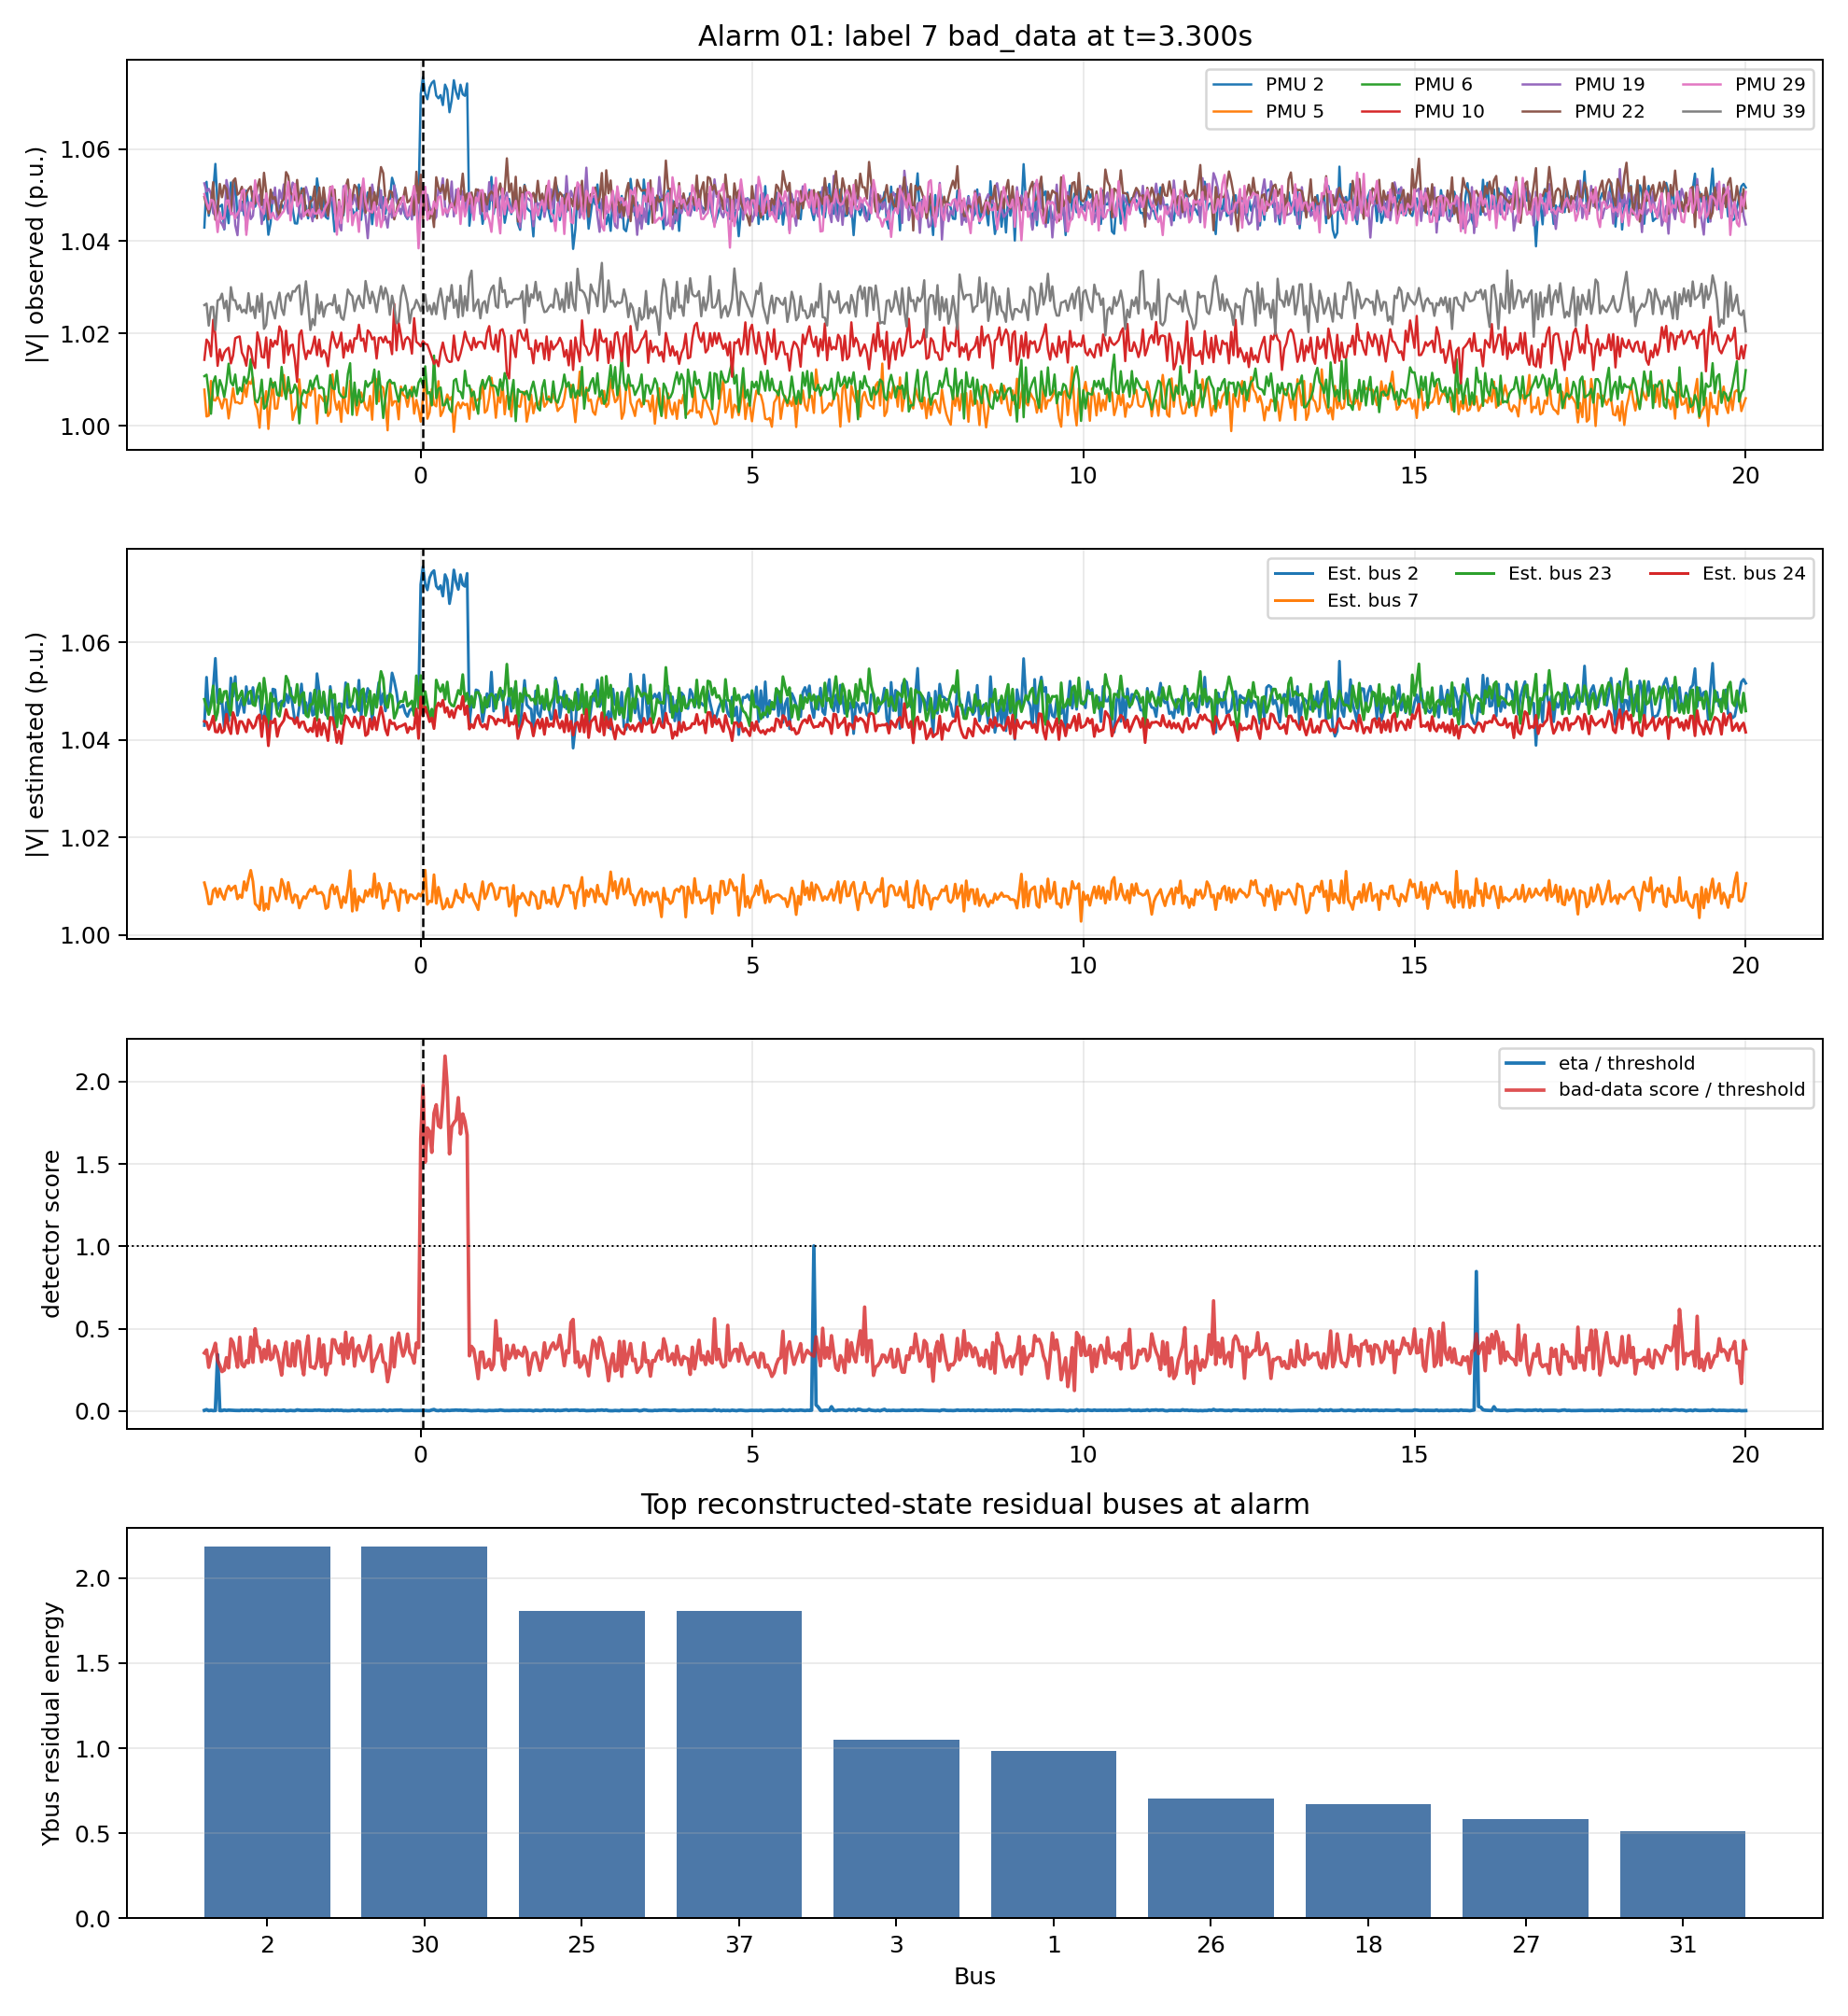
\includegraphics[width=0.92\linewidth]{engineering_review/figures/event_01_label7_bad_data.png}
  \caption{Label-7 bad data example. This is not a grid fault; it is a
  measurement-quality anomaly detected by three-phase inconsistency.}
  \label{fig:bad_data}
\end{figure}

\subsection{Example B: Bus 39 fault}

The Bus 39 fault creates a very large physical residual:
$\eta=5.29\times10^8$, or about $1.11\times10^5$ times the threshold. The
classifier predicts label 1 and the localizer returns Bus 39 as Top-1.

\begin{figure}[H]
  \centering
  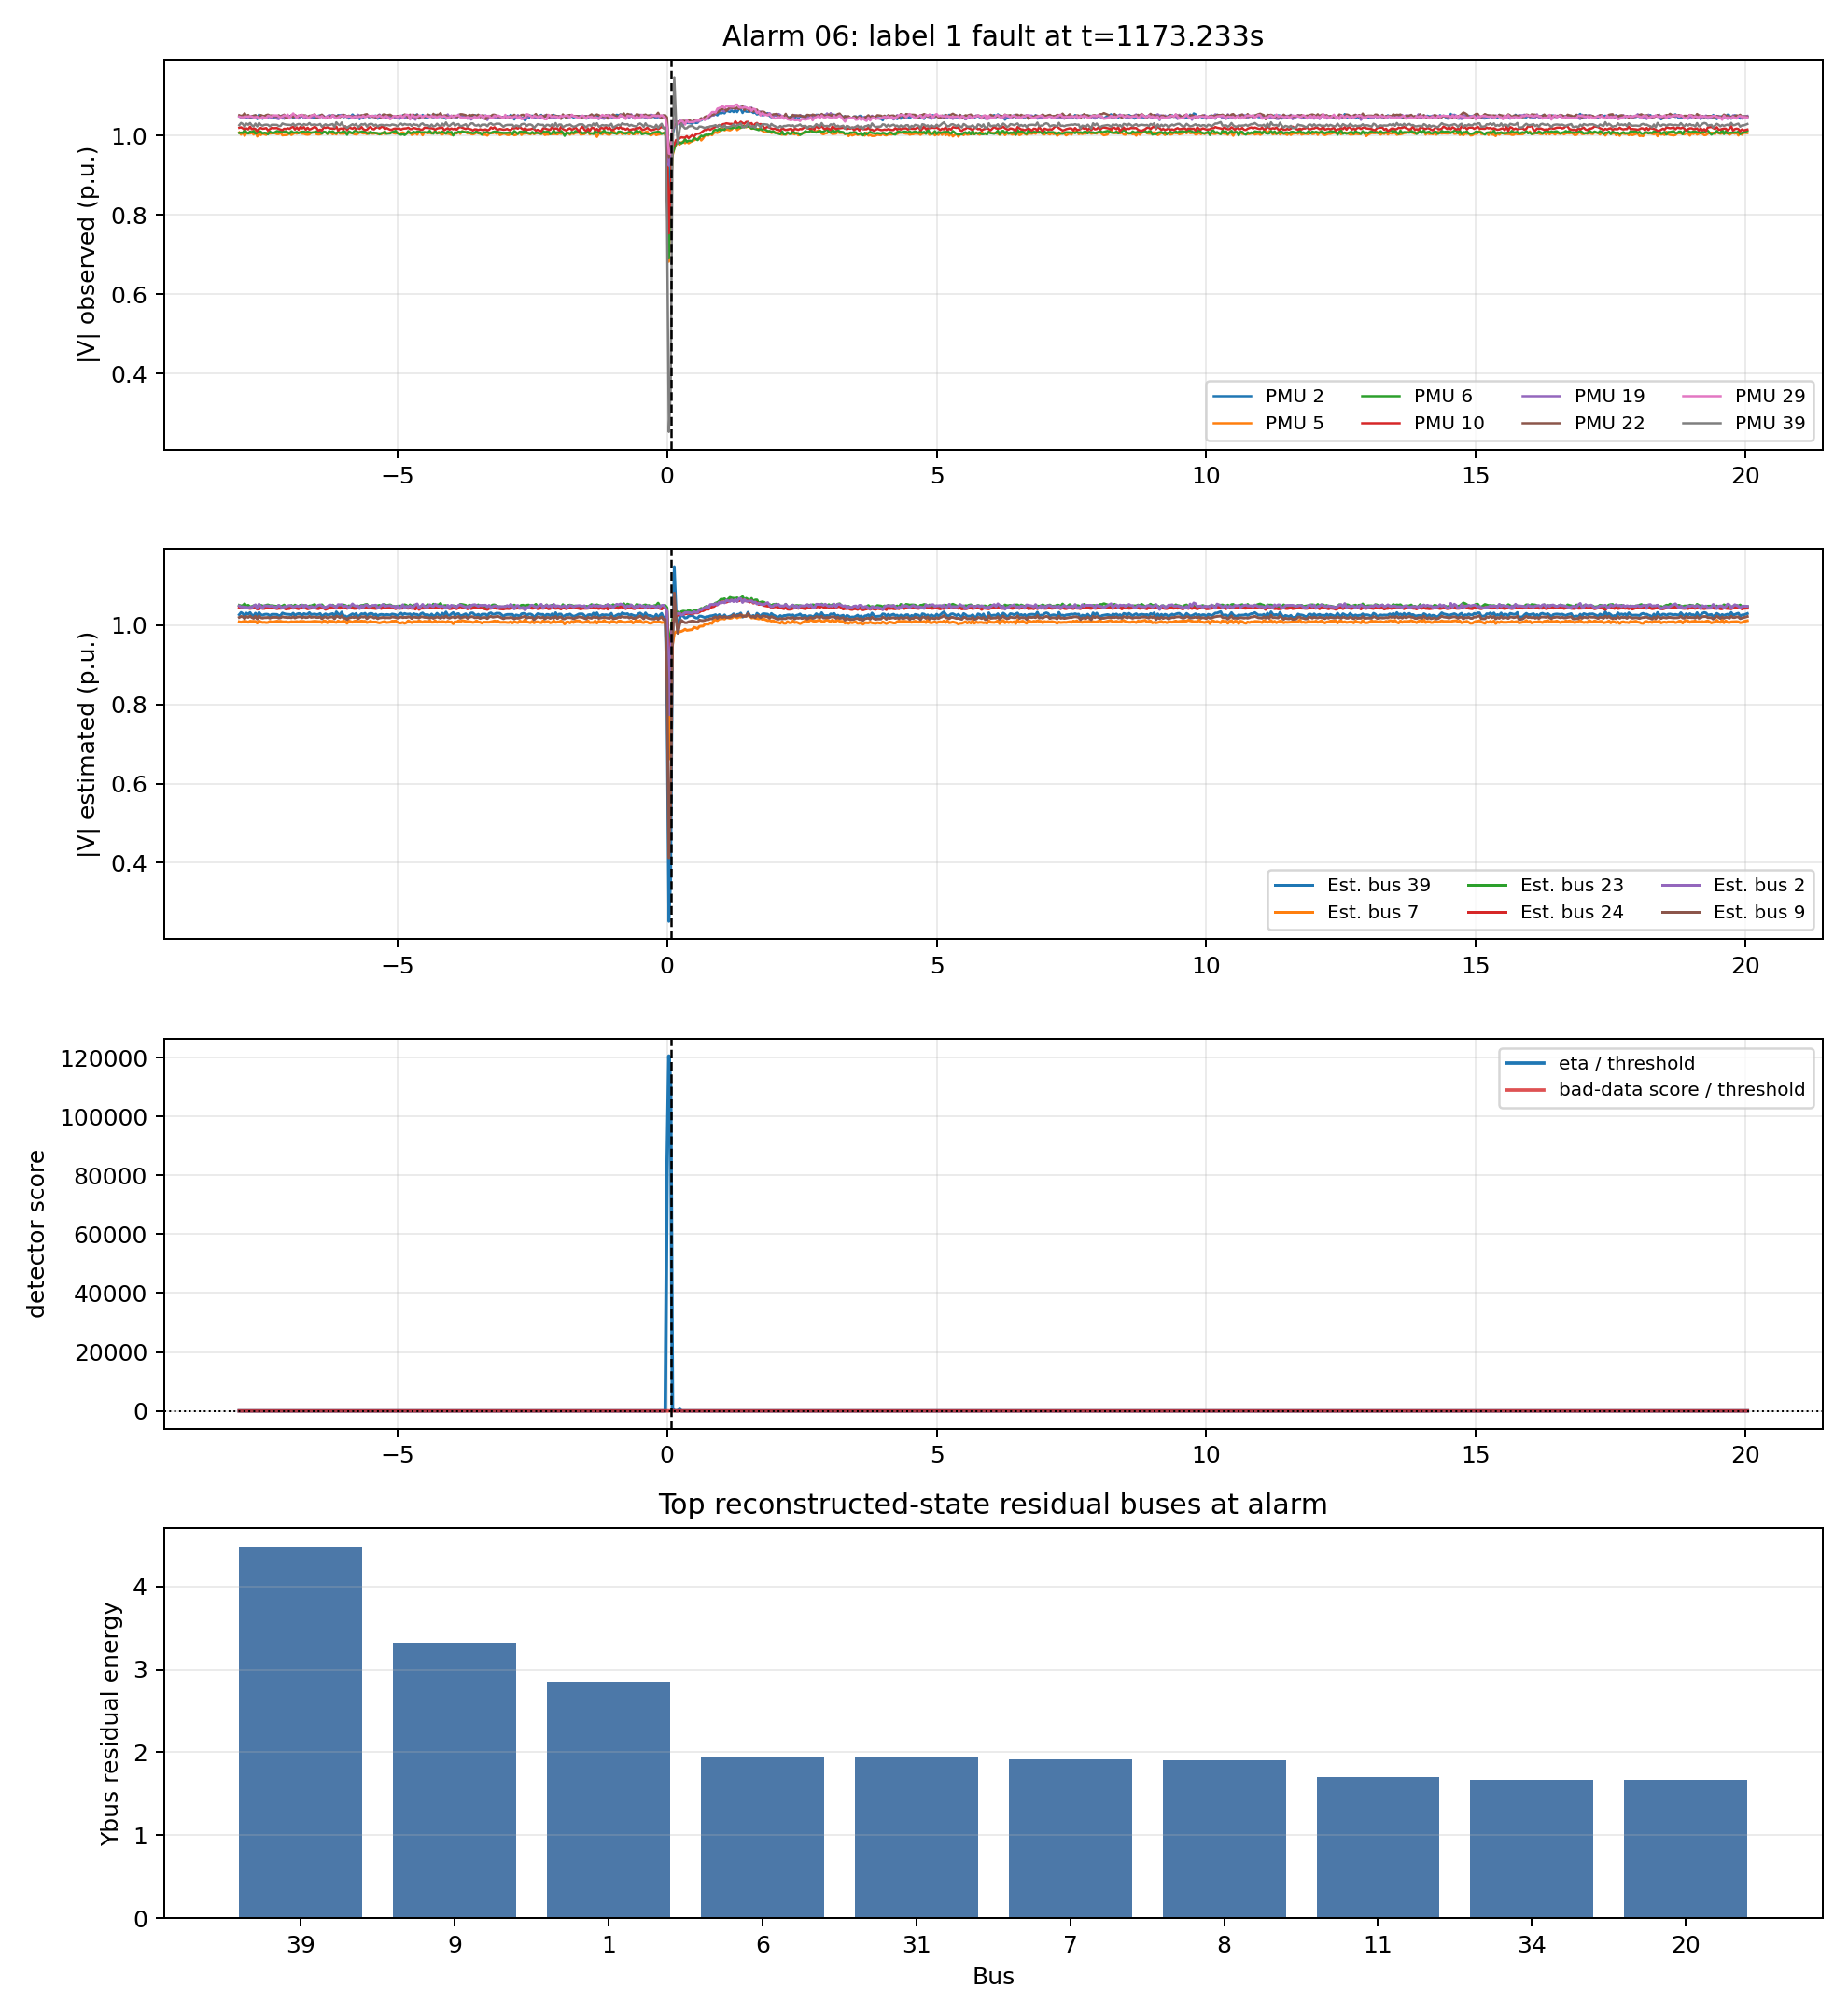
\includegraphics[width=0.92\linewidth]{engineering_review/figures/event_06_label1_fault.png}
  \caption{Bus 39 fault example. Large voltage/current residuals make this a
  high-confidence physical event.}
  \label{fig:fault}
\end{figure}

\subsection{Example C: Bus 24--23 line outage}

The line-outage alarm occurs at $t=39.588$ min with
$\eta=19146.03$, about 4.005 times the threshold. The classifier predicts label
2. The alarm-level bus endpoint is not perfect: the bus-valued Top-1 is Bus 35,
while the scheduled event is the Bus 24--23 line. This explains why localization
is 11/12 instead of 12/12. The line-candidate logic and report-side Top-3 line
review are retained because line events are inherently less naturally represented
by a single bus integer.

\begin{figure}[H]
  \centering
  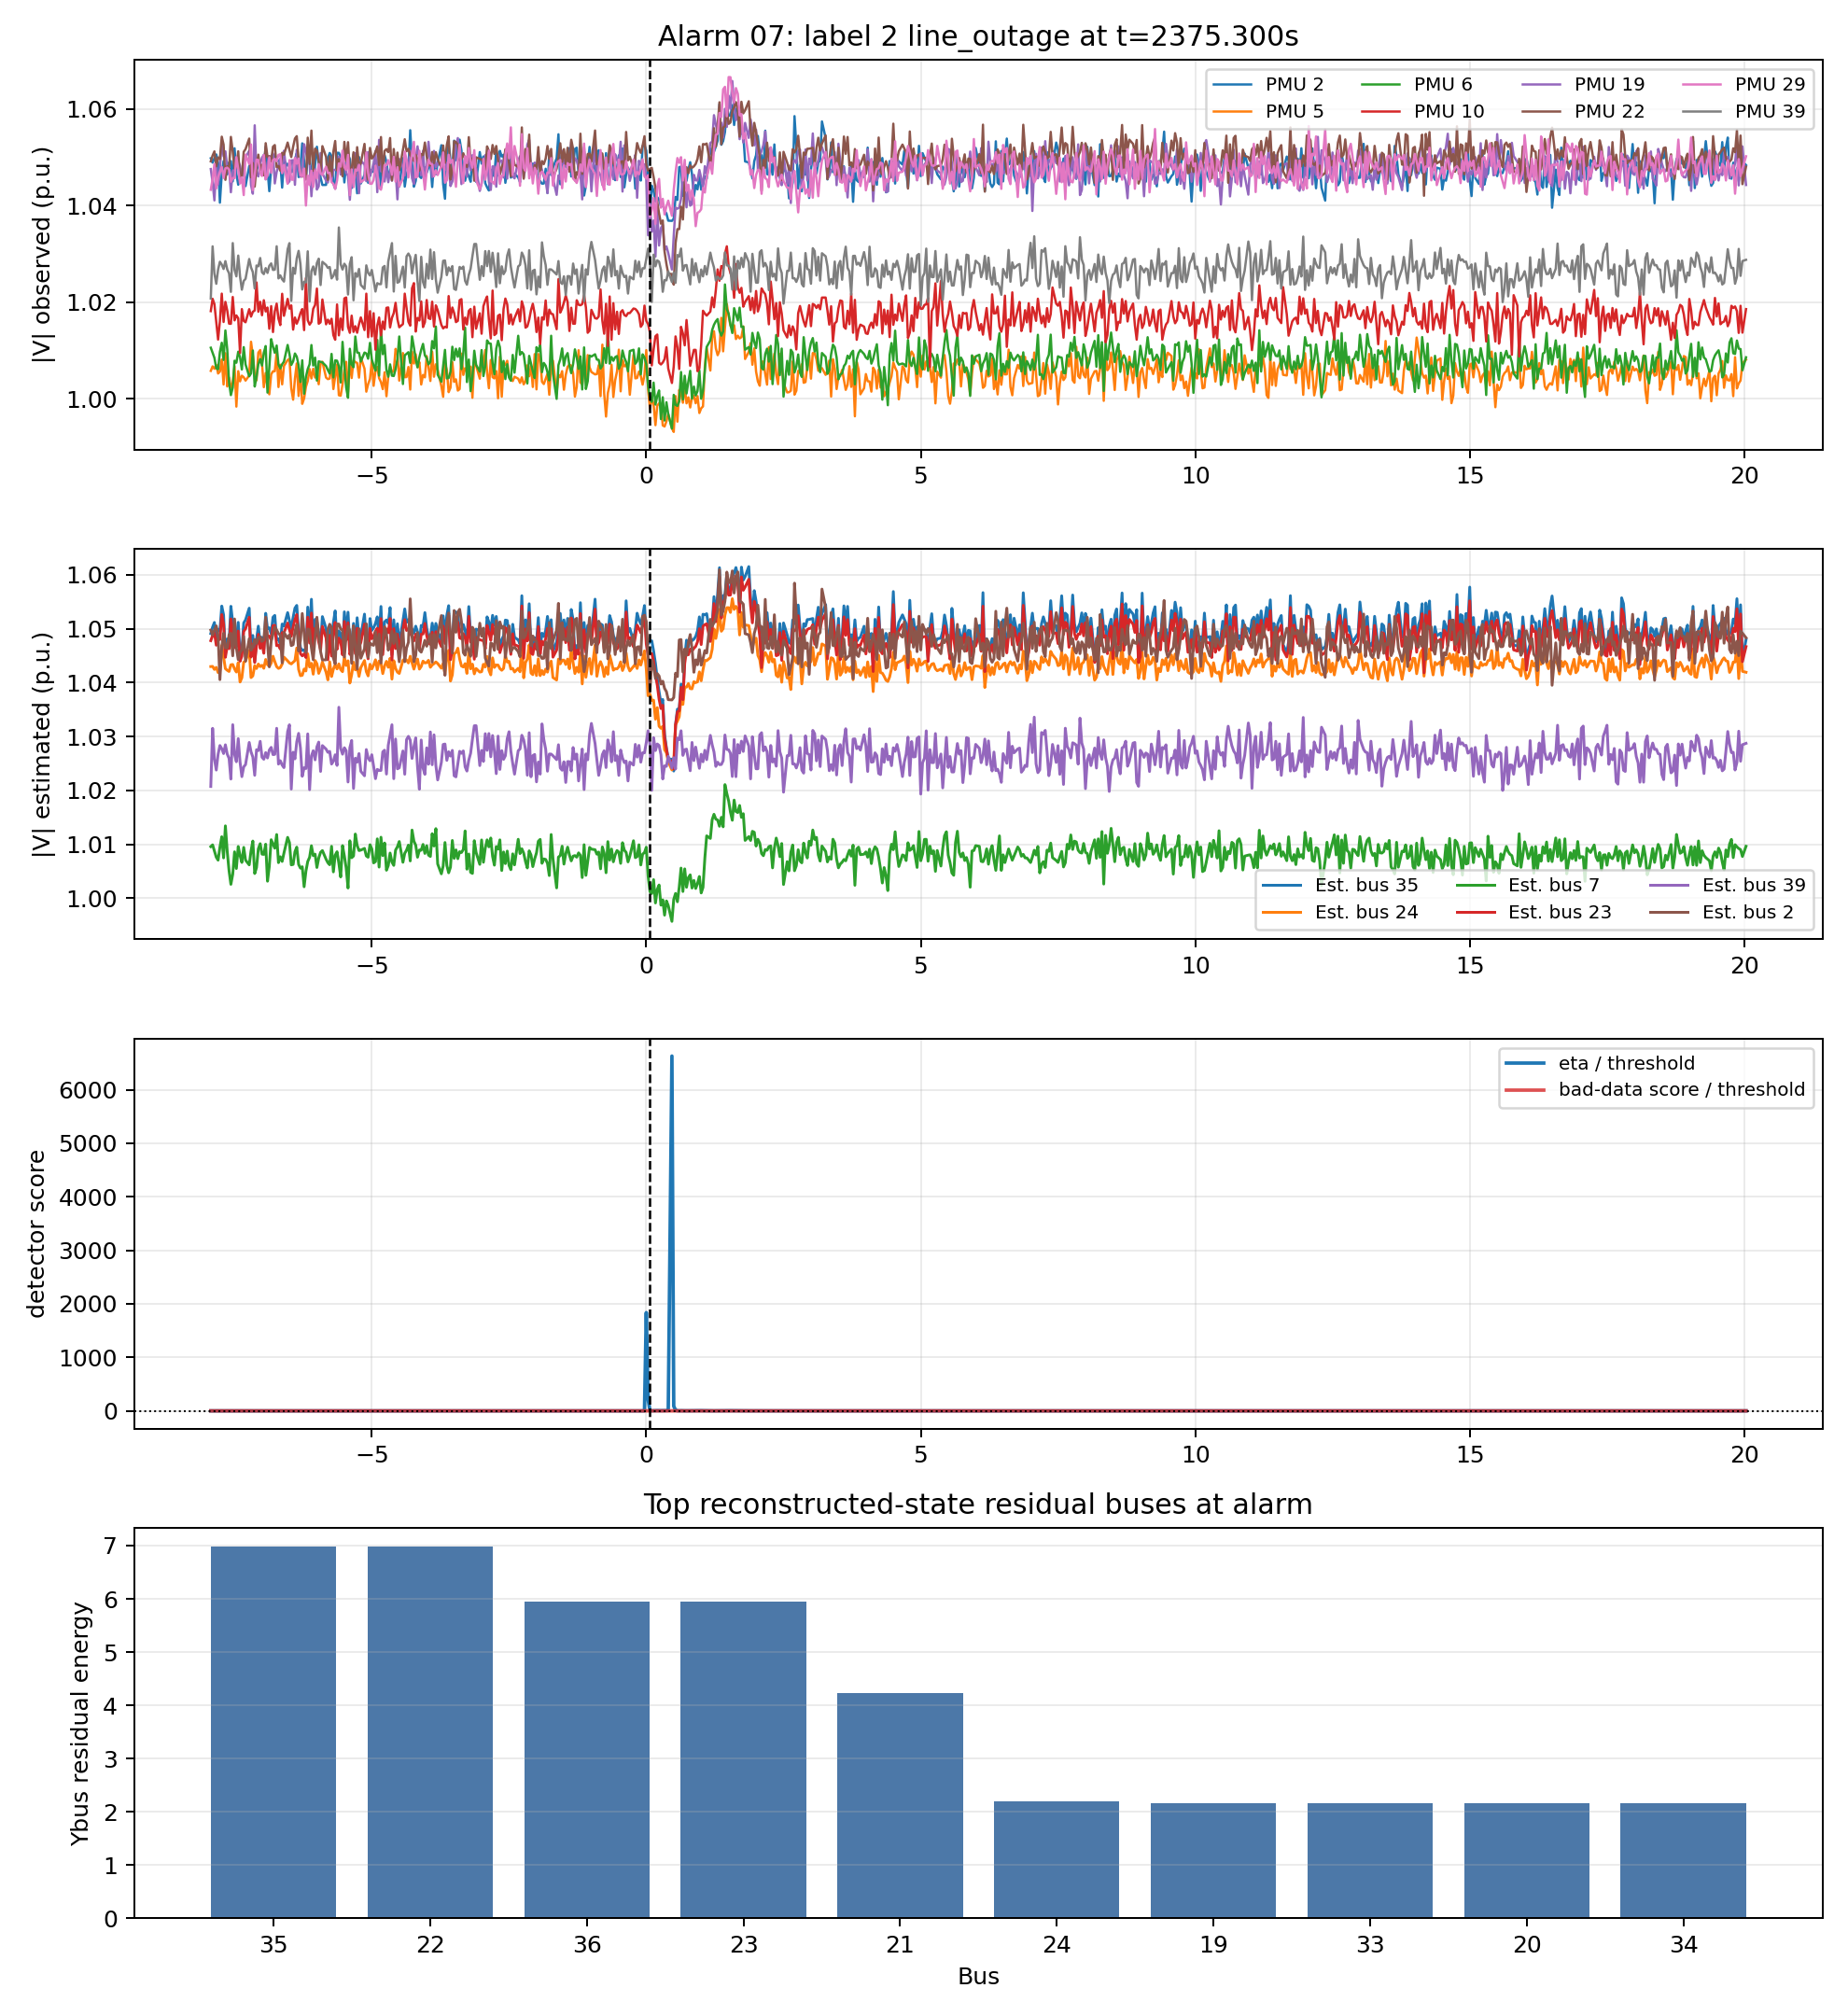
\includegraphics[width=0.92\linewidth]{engineering_review/figures/event_07_label2_line_outage.png}
  \caption{Line-outage example. The event is classified correctly, but
  bus-valued localization is the hardest part because a branch outage is not a
  single-bus phenomenon.}
  \label{fig:line_outage}
\end{figure}

\subsection{Example D: cyber+physical overlap}

At the 50-minute sequence, Bus 29 data becomes missing while a generation change
is visible in the remaining PMUs. The detector separates the sequence into
$5\rightarrow6\rightarrow3$. For the submission CSV, Bus 29 receives label 6
during the overlap, while non-missing PMUs receive the physical label 3 after the
overlap is isolated.

\begin{figure}[H]
  \centering
  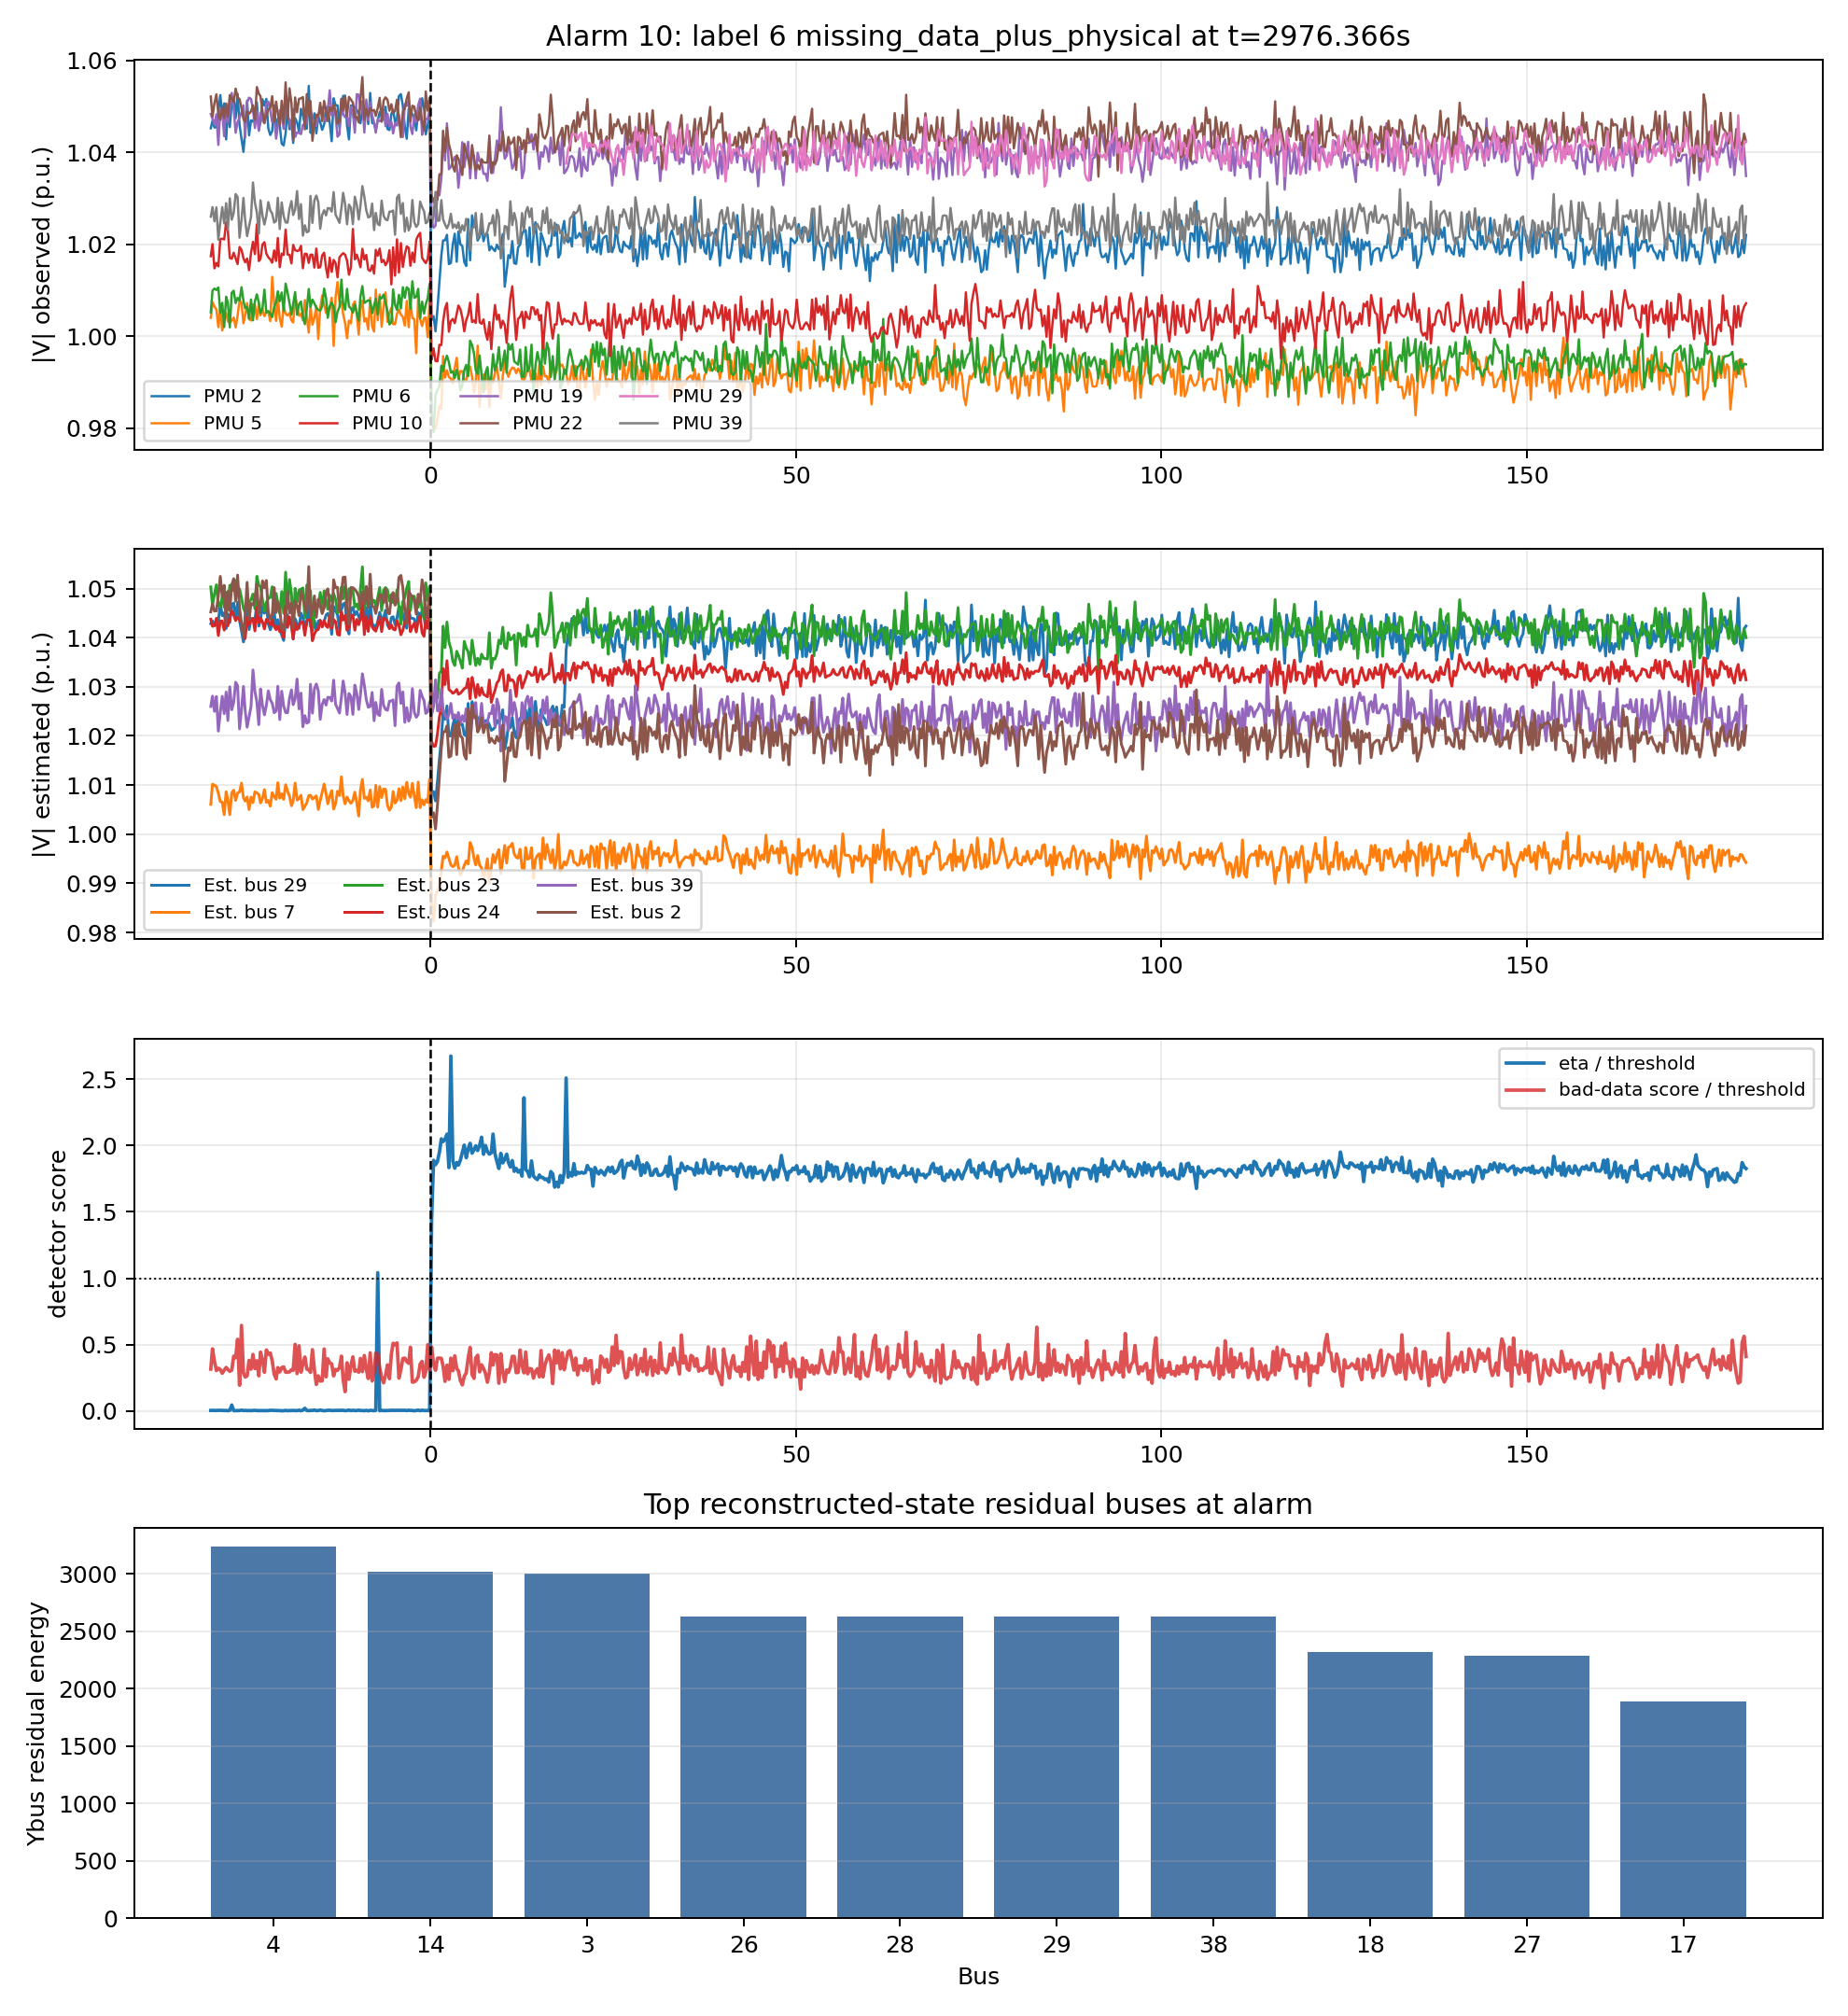
\includegraphics[width=0.92\linewidth]{engineering_review/figures/event_10_label6_missing_data_plus_physical.png}
  \caption{Cyber+physical overlap example. DATA\_PRESENT identifies the Bus 29
  communication failure, while the remaining PMUs carry the physical-generation
  signature.}
  \label{fig:cyber_physical}
\end{figure}

\subsection{Example E: Bus 2 generation change}

The generation-change alarm at $t=49.914$ min has $\eta=75991.8$, about 15.897
times the threshold. The classifier predicts label 3 and the localizer returns
Bus 2 as Top-1.

\begin{figure}[H]
  \centering
  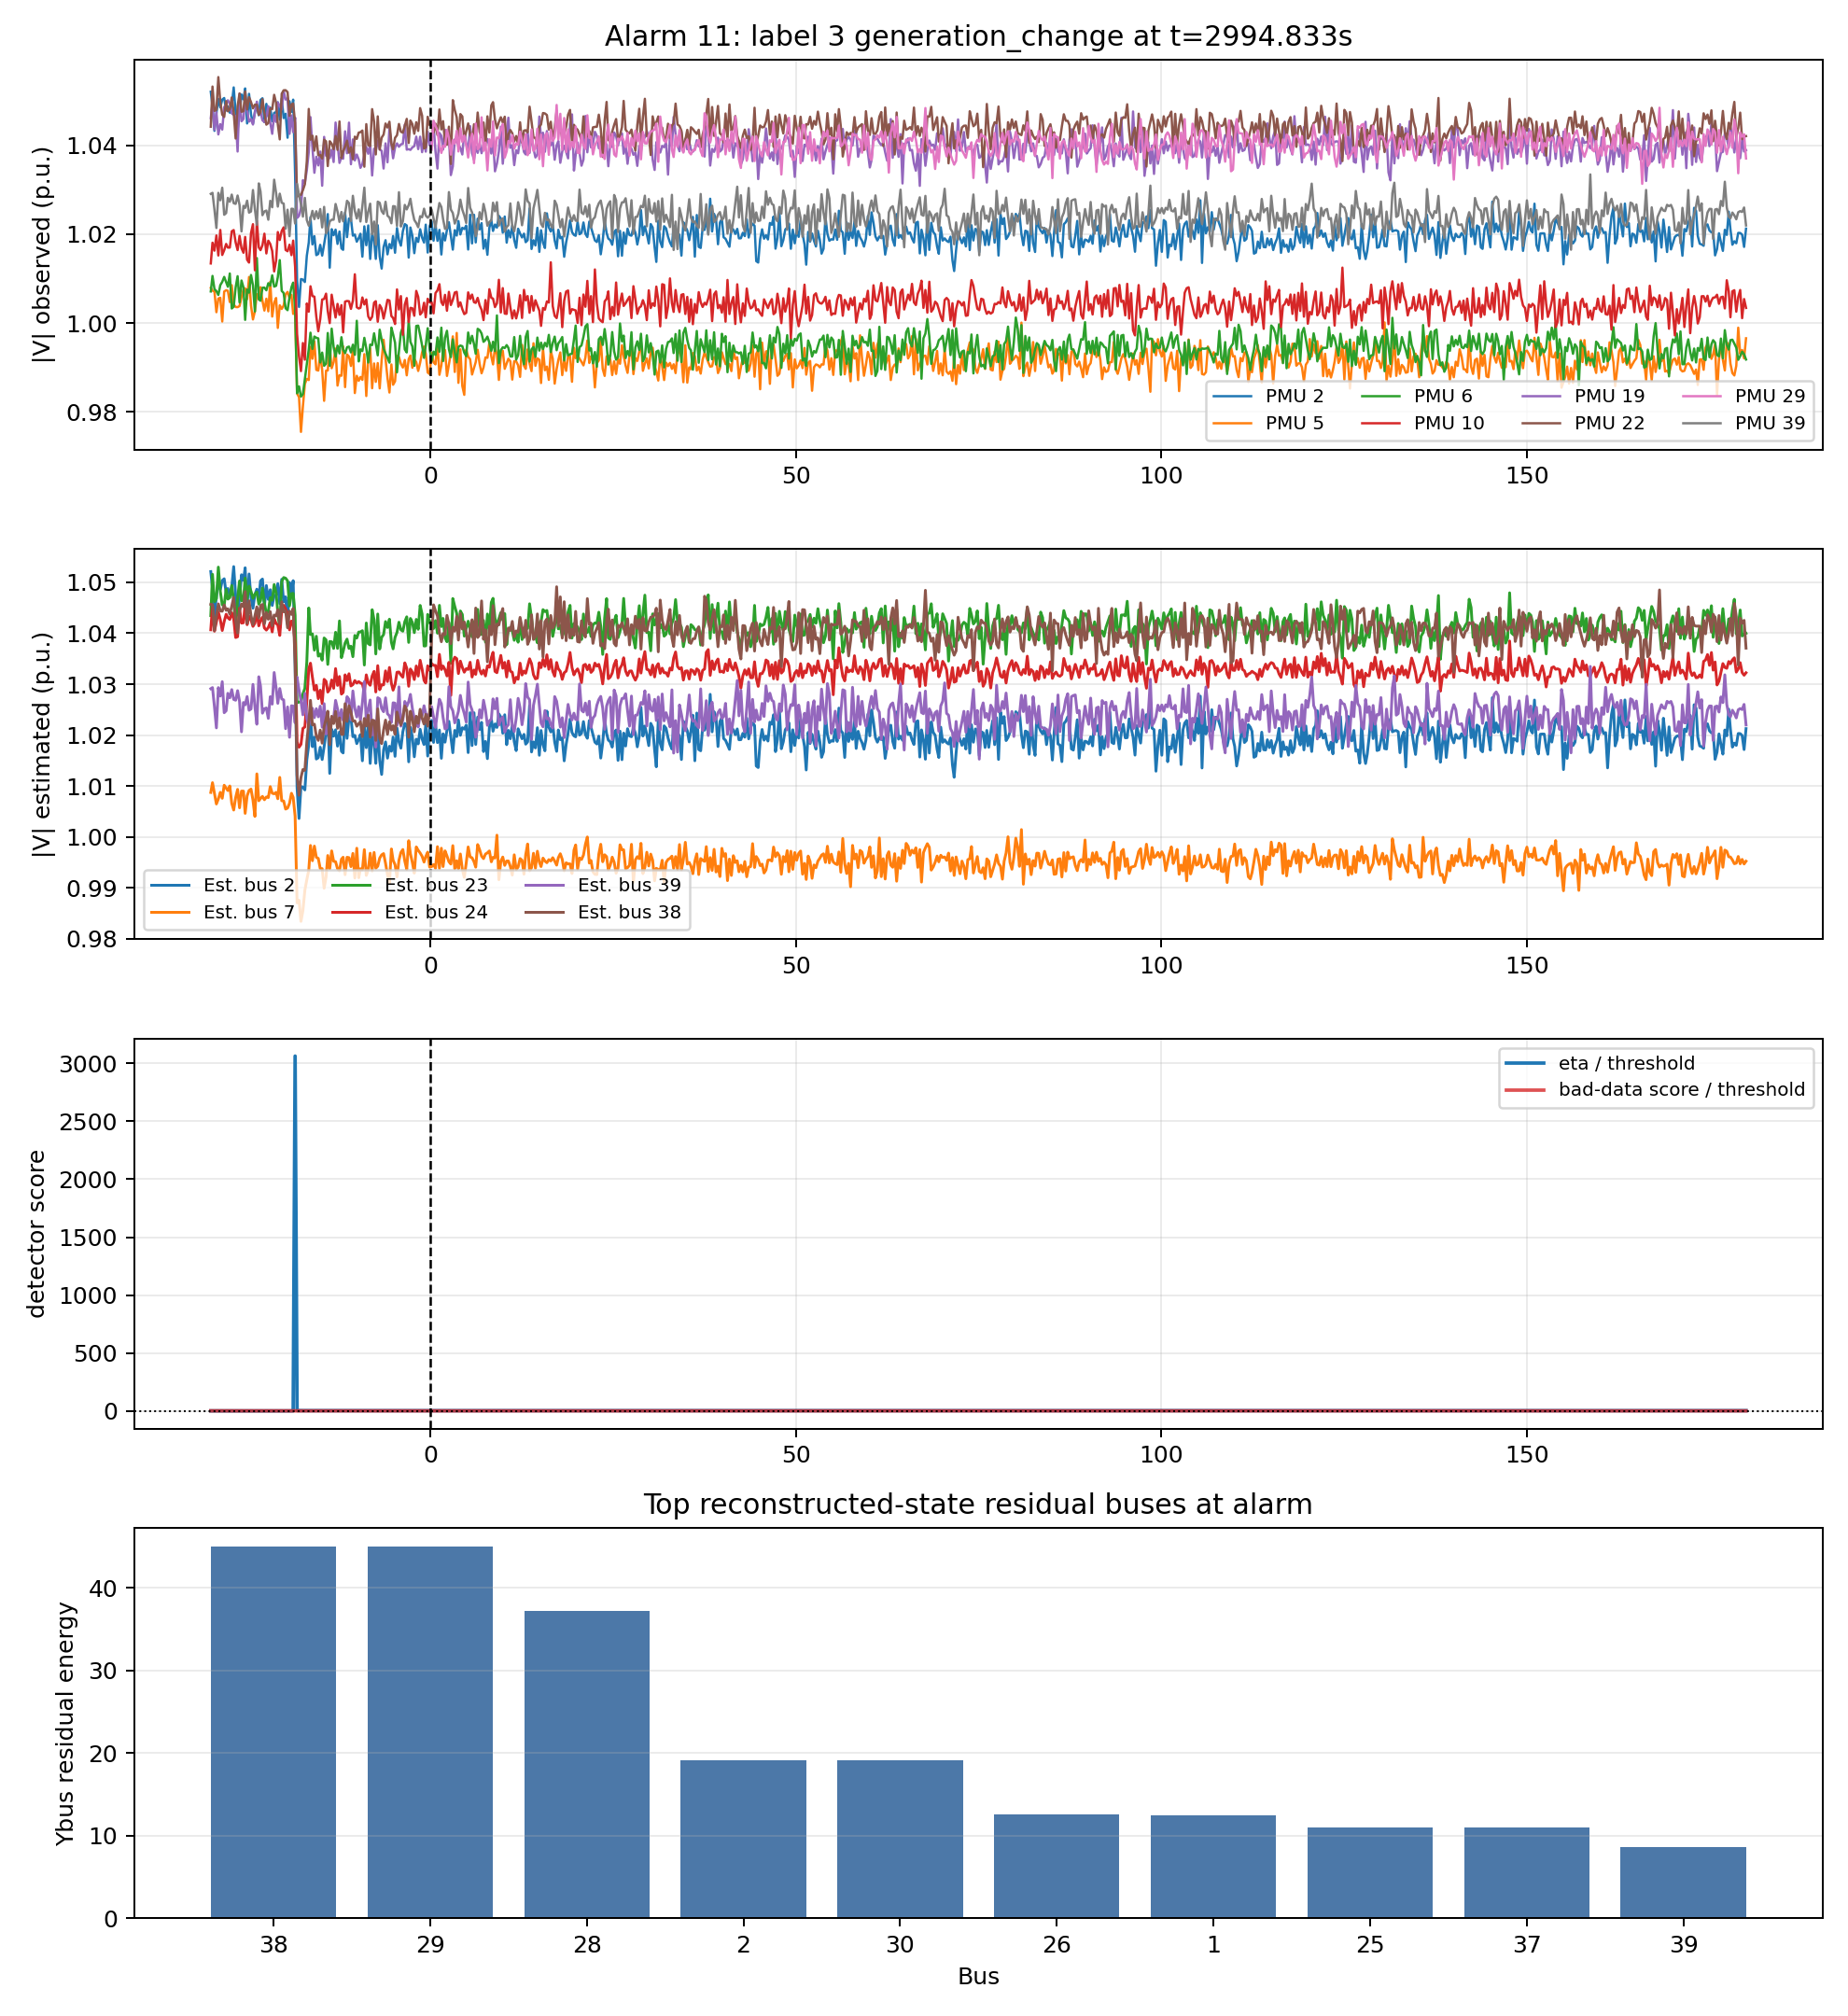
\includegraphics[width=0.92\linewidth]{engineering_review/figures/event_11_label3_generation_change.png}
  \caption{Bus 2 generation-change example. The event is visible after the
  cyber+physical sequence is split into separate transitions.}
  \label{fig:generation_change}
\end{figure}

\subsection{Example F: non-PMU Bus 7 load change}

Bus 7 has no PMU. The load-change alarm at $t=64.630$ min is therefore a direct
test of topology-aware localization. The detector statistic is modest but above
threshold: $\eta=5689.56$, about 1.19 times $\tau$. The classifier predicts label
4 and the Ybus/Jacobian localizer returns Bus 7 as Top-1.

\begin{figure}[H]
  \centering
  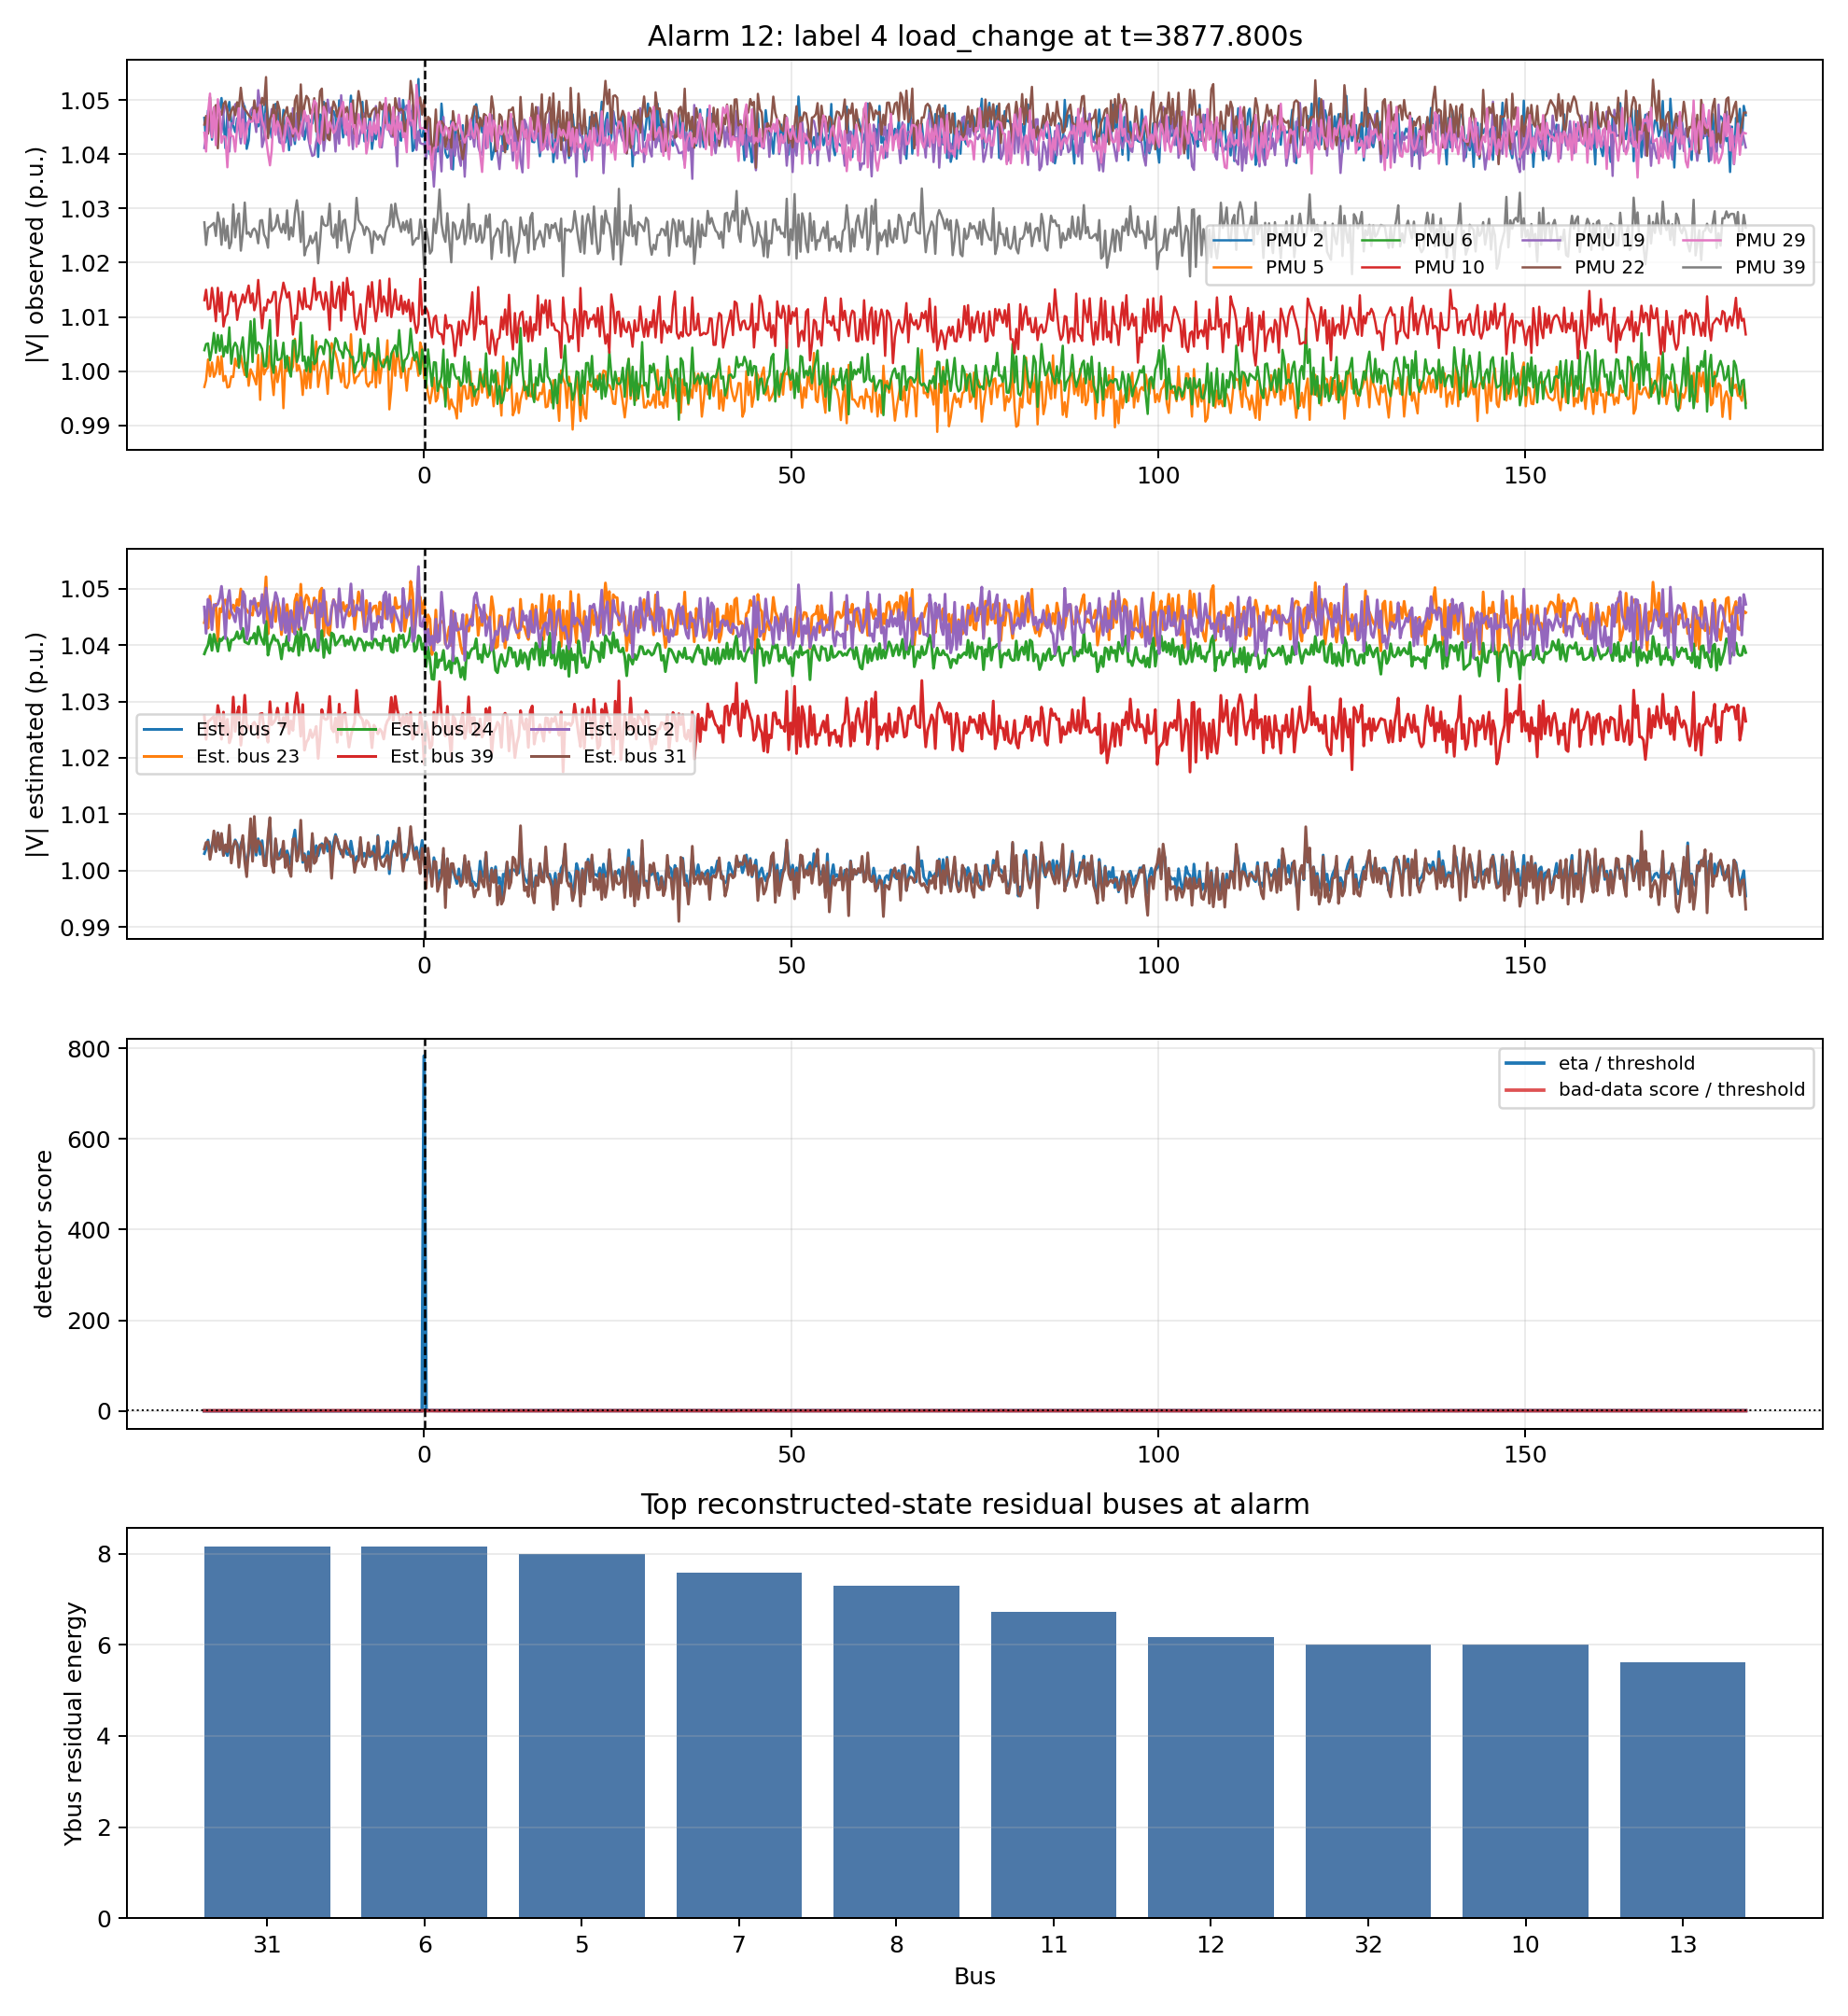
\includegraphics[width=0.92\linewidth]{engineering_review/figures/event_12_label4_load_change.png}
  \caption{Non-PMU Bus 7 load-change example. This is one of the key reasons for
  including the Ybus full-state proxy and targeted Bus 7 synthetic training
  scenarios.}
  \label{fig:load_change}
\end{figure}

\section{Row-Level Submission Semantics}

Alarm detection is onset-oriented: it should fire quickly. The competition CSV,
however, is row-oriented: it needs a label at every timestamp. The final writer
therefore expands alarm onsets into intervals using transparent rules.

\begin{table}[H]
\centering
\caption{Row-level interval writing rules.}
\begin{tabular}{p{0.25\linewidth}p{0.66\linewidth}}
\toprule
Predicted label & Row-level writing rule \\
\midrule
Fault, label 1 & Short physical interval, default 5 s unless interrupted. \\
Line outage, label 2 & Short physical interval, default 5 s unless interrupted;
location stores a deterministic bus endpoint. \\
Generation change, label 3 & Persistent physical interval, default 5 min unless
another onset interrupts it. \\
Load change, label 4 & Persistent physical interval, default 5 min unless another
onset interrupts it. \\
Missing data, label 5 & Written only where the PMU's own DATA\_PRESENT flag is 0. \\
Cyber+physical, label 6 & Written on the missing PMU; non-missing PMUs retain the
physical component. \\
Bad data, label 7 & Written only to the localized corrupted PMU. \\
Unknown, label 8 & Supported by schema, but no visible label-8 examples exist. \\
\bottomrule
\end{tabular}
\label{tab:writer_rules}
\end{table}

This bus-aware writer is important. If label 5 or 6 were copied to all PMU files,
the submission would claim that all PMUs were missing even when only Bus 29 was
down. That would be physically wrong and would reduce sample-level agreement
with the per-PMU \Event{} columns.

\section{Final Metrics in Detail}

\subsection{Event-level alarm metrics}

The event-level alarm table is intentionally separated from sample-level metrics.
It answers: did the system raise a timely alarm for each visible transition?

\begin{table}[H]
\centering
\caption{Final alarm-level detection and classification.}
\begin{tabular}{lcl}
\toprule
Metric & Value & Interpretation \\
\midrule
Base detector F1 & 0.857 & Physical/cyber detector misses short bad-data bursts \\
Final detection precision & 1.000 & No unmatched visible alarms \\
Final detection recall & 1.000 & All 12 visible transitions matched \\
Final detection F1 & 1.000 & Consequence of 12 TP, 0 FP, 0 FN \\
FP/min & 0.000 & No false alarms over the 90-minute public file \\
Mean delay & 0.0475 s & First correct alarm after visible transition \\
Classification macro-F1 & 1.000 & Matched alarm labels 1--7 correct \\
Classification weighted-F1 & 1.000 & Same, weighted by matched support \\
\bottomrule
\end{tabular}
\label{tab:alarm_metrics}
\end{table}

\subsection{Sample-level metrics}

Sample-level metrics ask a stricter question: did every row in every PMU file
receive the right label? This is harder because event duration must be inferred.

\begin{table}[H]
\centering
\caption{Sample-level confusion matrix aggregated over all eight PMU files. Rows are true labels and columns are predicted labels.}
\scriptsize
\begin{tabular}{c|rrrrrrrrr}
 &0&1&2&3&4&5&6&7&8\\
\hline
0&1130372&24&208&208&0&0&0&17&0\\
1&16&1176&0&0&0&0&0&0&0\\
2&16&0&992&0&0&0&0&0&0\\
3&0&0&0&75670&0&0&0&0&0\\
4&1056&0&0&0&72000&0&0&0&0\\
5&0&0&0&0&0&8646&0&0&0\\
6&0&0&0&0&0&0&554&0&0\\
7&4&0&0&0&0&0&0&73&0\\
8&0&0&0&0&0&0&0&0&0\\
\end{tabular}
\label{tab:confusion}
\end{table}

The confusion matrix shows why the system is strong but not literally perfect.
Label 5 and label 6 are exact on visible rows. Label 3 is exact on visible rows
after the 50-minute split. Label 4 has 1056 rows scored as normal, mainly due to
duration-boundary mismatch around persistent load-change intervals. Label 8 has
zero support, so macro-F1 over 0--8 includes a zero-F1 class.

\begin{table}[H]
\centering
\caption{Bus-aware prediction support per PMU file.}
\scriptsize
\begin{tabular}{lrrrrrrrr}
\toprule
Bus file & 0 & 1 & 2 & 3 & 4 & 5 & 6 & 7\\
\midrule
Bus2 & 142495 & 150 & 150 & 9554 & 9000 & 0 & 0 & 30\\
Bus5 & 142525 & 150 & 150 & 9554 & 9000 & 0 & 0 & 0\\
Bus6 & 142525 & 150 & 150 & 9554 & 9000 & 0 & 0 & 0\\
Bus10 & 142525 & 150 & 150 & 9554 & 9000 & 0 & 0 & 0\\
Bus19 & 142525 & 150 & 150 & 9554 & 9000 & 0 & 0 & 0\\
Bus22 & 142525 & 150 & 150 & 9554 & 9000 & 0 & 0 & 0\\
Bus29 & 133879 & 150 & 150 & 9000 & 9000 & 8646 & 554 & 0\\
Bus39 & 142465 & 150 & 150 & 9554 & 9000 & 0 & 0 & 60\\
\bottomrule
\end{tabular}
\label{tab:bus_support}
\end{table}

\section{Leakage and Numerical-Bug Audit}

This project was specifically reviewed for reasons why the high numbers might be
untrustworthy.

\subsection{Potential issue found and fixed}

The suspicious pattern was detector calibration. If the detector threshold is
calibrated using \texttt{Event == 0}, then the detector has indirectly used the
answer key to decide what is normal. That can inflate metrics. The final code
fixes this:

\begin{itemize}
  \item \texttt{src/classifier/train\_lgbm.py} builds the detector from first-60
  second robust candidates and does not use Event labels.
  \item \texttt{src/estimator/calibration.py} accepts an explicit
  \texttt{calibration\_mask}; when supplied, it does not inspect Event.
  \item The final report and JSON explicitly state that Event is used for scoring
  and supervised classifier labels, not detector firing or detector calibration.
\end{itemize}

\subsection{Other checks}

\begin{table}[H]
\centering
\caption{Final quality checks.}
\begin{tabular}{ll}
\toprule
Check & Result \\
\midrule
Full tests & 214 passed, 1 expected xfail, exit code 0 \\
Prediction validation & ok: true \\
Per-bus row count & 161379 rows each \\
Combined submission rows & $8\times161379$ \\
Timestamp alignment & pass for all eight PMU files \\
Valid labels & only 0--7 present, label 8 supported but not predicted visibly \\
Valid locations & -1 or bus 1--39 \\
Engineering review figures & 13 PNG files \\
Engineering review JSON & detection audit, per-bus metrics, units, topology \\
ZIP audit & 106 files, 0 forbidden bytecode/cache/LaTeX auxiliary files \\
\bottomrule
\end{tabular}
\label{tab:audit}
\end{table}

\section{What Could Still Fail on Hidden Data?}

The report should be honest about residual risks:

\begin{enumerate}
  \item \textbf{Label 8 open-set behavior}: no visible label-8 examples exist.
  The system supports label 8 in schema but does not claim high confidence for
  unseen unknown-event behavior.
  \item \textbf{Duration mismatch}: generation/load events are expanded using
  visible-data duration priors. Hidden events could last longer or shorter.
  \item \textbf{Line localization}: branch outages are less naturally represented
  by a single bus-valued \PredLoc{} field. The report keeps line Top-3 details in
  JSON, but the official CSV stores a deterministic endpoint.
  \item \textbf{Sparse PMU observability}: the Ybus proxy is a topology-consistent
  estimator, not a full nonlinear dynamic state observer. It is useful for
  localization features, but it cannot perfectly reconstruct every hidden-bus
  transient.
  \item \textbf{Visible-event count}: a 1.000 alarm metric over 12 transitions is
  meaningful but statistically limited. Hidden scoring could expose cases absent
  from the visible file.
\end{enumerate}

\section{Conclusion}

The final submission is a strong, physics-informed, auditable solution. It uses
all eight PMUs jointly, handles PMU-specific cyber and bad-data semantics,
uses topology and Ybus to reason about non-PMU buses, targets the known hard
cases with synthetic data, and includes engineering-review artifacts that explain
each alarm. The 1.000 detection score is not a magic claim: it follows from 12
visible true positives, zero false positives, and zero false negatives under the
chosen visible-transition audit. The more complete picture is that the system is
excellent on visible detection/classification, strong but not perfect on
sample-level and localization details, and transparent about hidden-test risks.

\section*{Artifact Index}

\begin{itemize}
  \item \texttt{predictions/}: eight per-bus prediction CSVs plus combined
  \texttt{submission.csv}.
  \item \texttt{report/sgsma2026\_report.pdf}: compiled version of this report.
  \item \texttt{report/engineering\_review/detection\_and\_scenario\_audit.json}:
  alarm-by-alarm audit.
  \item \texttt{report/engineering\_review/per\_bus\_sample\_metrics.json}:
  bus-specific Event-column metrics.
  \item \texttt{report/engineering\_review/units.json}: units and output-field
  definitions.
  \item \texttt{report/engineering\_review/ieee39\_topology.json}: topology,
  PMU flags, branches, and deterministic layout coordinates.
  \item \texttt{report/engineering\_review/figures/}: topology and alarm plots.
  \item \texttt{report/model\_benchmark.csv} and
  \texttt{report/model\_benchmark.json}: ten-model compact benchmark outputs.
  \item \texttt{report/localization\_explanations.json}: per-alarm Ybus/Zbus,
  Jacobian, and PMU-direct localization evidence.
  \item \texttt{experiments/event\_simulations/}: seven label-specific
  simulation bundles with metadata, plots, and PMU CSVs.
  \item \texttt{experiments/andes\_fault\_bus7/}: ANDES Bus 7 reconstruction
  experiment.
\end{itemize}

\begin{thebibliography}{00}
\bibitem{kundur}
P. Kundur, \textit{Power System Stability and Control}. McGraw-Hill, 1994.

\bibitem{andes}
H. Cui, F. Li, and K. Tomsovic, ``ANDES: A Python-based cyber-physical power
system simulation tool,'' \textit{IEEE Transactions on Power Systems}, 2021.

\bibitem{basseville}
M. Basseville and I. Nikiforov, \textit{Detection of Abrupt Changes: Theory and
Application}. Prentice-Hall, 1993.

\bibitem{lightgbm}
G. Ke et al., ``LightGBM: A highly efficient gradient boosting decision tree,''
in \textit{Advances in Neural Information Processing Systems}, 2017.
\end{thebibliography}

\end{document}
